\documentclass{cumcm}
\usepackage{array}
\newcommand{\PreserveBackslash}[1]{\let\temp=\\#1\let\\=\temp}
\newcolumntype{C}[1]{>{\PreserveBackslash\centering}p{#1}}
\newcolumntype{R}[1]{>{\PreserveBackslash\raggedleft}p{#1}}
\newcolumntype{L}[1]{>{\PreserveBackslash\raggedright}p{#1}}

% \title{text}这里是显示在第三页的文章标题
\title{基于的目标规划模型的系泊系统设计}
% \displaytitle{text} 这里是显示在承诺书上的文章标题,注意,不能换行,如果题目特别长,要进行适当的缩写
\displaytitle{基于的目标规划模型的系泊系统设计}
% \school{text}命令用于在承诺书上显示学校名称。按要求,此处应填写全称
\school{上海交通大学}
% 以下命令分别显示队员、指导教师姓名以及队伍编号
\authorone{}
\authortwo{}
\authorthree{}
\advisor{}
\teamnumber{}

\begin{document}

% 这里用于打印承诺书以及编号页
 
%\newpage
\thispagestyle{empty} %取消当前页码
{\Large \heiti \begin{center}\the\year~高教社杯全国大学生数学建模竞赛\par\vspace{0.5\ccwd}\par
{\ziju{1}承诺书}\end{center}\par\vspace{1\ccwd}\par}
\renewcommand{\baselinestretch}{1.5}\normalsize
{\zihao{-4}%
我们仔细阅读了中国大学生数学建模竞赛的竞赛规则。\par
我们完全明白,在竞赛开始后参赛队员不能以任何方式(包括电话、电子邮件、网上咨询等)
与队外的任何人(包括指导教师)研究、讨论与赛题有关的问题。\par
我们知道,抄袭别人的成果是违反竞赛规则的, 如果引用别人的成果或其他公开的资料
(包括网上查到的资料),必须按照规定的参考文献的表述方式在正文引用处和参考文献中明确列出。\par
我们郑重承诺,严格遵守竞赛规则,以保证竞赛的公正、公平性。如有违反竞赛规则的行为,我们将受到严肃处理。\par
\par\vspace{2\ccwd}\par
\raisebox{1ex}[0pt]{我们参赛的题目是:}\vbox{\hbox to11.4cm{\hfil \the\displaytitle \hfil}
        \protect\vspace{0.6truemm}\relax
        \hrule depth0pt height0.15truemm width11.4cm}\par
\vspace{1mm}
\raisebox{1ex}[0pt]{我们的参赛报名号为(如果赛区设置报名号的话):}\vbox{\hbox to5.75cm{\hfil \the \teamnumber  \hfil}
        \protect\vspace{0.6truemm}\relax
        \hrule depth0pt height0.15truemm width5.75cm}\par
\vspace{1mm}
\raisebox{1ex}[0pt]{所属学校(请填写完整的全名):}\vbox{\hbox to9.12cm{\hfill \the\school \hfill}
        \protect\vspace{0.6truemm}\relax
        \hrule depth0pt height0.15truemm width9.12cm}\par
\begin{tabular}{lcp{8.82cm}c}
\hspace{-2.1mm}\raisebox{-1mm}[0pt]{参赛队员(打印并签名): }&\raisebox{-1mm}[0pt]{1、}& \raisebox{-1mm}[0pt]{\the\authorone\hfill{}}& \\ \cline{3-3}
   &\raisebox{-1mm}[0pt]{2、}& \raisebox{-1mm}[0pt]{\the\authortwo\hfill{}}& \\ \cline{3-3}
   &\raisebox{-1mm}[0pt]{3、}& \raisebox{-1mm}[0pt]{\the\authorthree\hfill{}}& \\ \cline{3-3}
\end{tabular}
\par
\vspace{10mm}
\raisebox{1ex}[0pt]{指导教师或指导教师组负责人(打印并签名):}\vbox{\hbox to6.65cm{\the\advisor \hfil}
        \protect\vspace{0.6truemm}\relax
        \hrule depth0pt height0.15truemm width6.65cm}\par
\vspace{5mm}
{}\hspace{10cm}日期:\hrulefill\hrulefill 年\hrulefill 月 \hrulefill 日
\par
\vspace{2cm}
\hrulefill\par\vspace{2\ccwd}\par
赛区评阅编号(由赛区组委会评阅前进行编号):
}
\renewcommand{\baselinestretch}{1.3}\normalsize
\newpage
\thispagestyle{empty} %取消当前页码
{\Large \heiti \begin{center}\the\year~高教社杯全国大学生数学建模竞赛\par\vspace{0.5\ccwd}\par
{\ziju{1}编号专用页}\end{center}\par\vspace{1\ccwd}\par}
{\zihao{-4}%
\par\vfill
赛区评阅编号(由赛区组委会评阅前进行编号):\par\vfill\vfill

赛区评阅记录(可供赛区评阅时使用):\vspace{1\ccwd}

\begin{center}
\resizebox{.9\textwidth}{!}{
\begin{tabular}{|c|*{10}{p{.09\textwidth}|}}
\hline
\makecell{评\\阅\\人}&&&&&&&&&&\\
\hline
\makecell{评\\分}&&&&&&&&&&\\
\hline
\makecell{备\\注}&&&&&&&&&&\\
\hline
\end{tabular}
}
\end{center}\vspace{1\ccwd}

全国统一编号(由赛区组委会送交全国前编号):\par\vfill\vfill

全国评阅编号(由全国组委会评阅前进行编号):\par\vfill\vfill\vfill
}
\renewcommand{\baselinestretch}{1.3}\normalsize

\newpage

\begin{minipage}{0.9\textwidth}
\centering\LARGE\textbf{基于的目标规划模型的系泊系统设计}
\end{minipage}

\setcounter{page}{1}
\begin{abstract}
本题意在考察分析系泊系统在不同的外界环境参数影响下工作状态的变化情况,进而对重物球质量参数进行调整,完成系泊系统的设计以满足一定的工作条件,使得该系统能够达到预期的工作效果。\par
\textbf{针对问题一}\quad 建立二维平面内的力学模型,以浮标的受力为切入点,按照自上而下的顺序,对系泊系统的各个组成部分进行递推式受力分析。对于锚链建立悬链线模型,悬链线模型中的坐标方程与力学平衡方程相联立,从而得出各物理量数值。由于锚链根据风力大小不同可能出现两种情况,锚链全部浮起以及锚链部分沉底。为此我们分情况进行了讨论。计算结果为:风速为$12m/s$时,钢桶倾斜角$1.0083^\circ$,吃水深度$0.7348m$,游动半径$14.3061m$,沉底长度$6.8219m$,锚链参数$3.3198$;风速为$24m/s$时,钢桶倾斜角$3.8498^\circ$,吃水深度$0.7489m$,游动半径$17.4255m$,沉底长度$0.3158m$,锚链参数$13.3108$。\par
\textbf{针对问题二}\quad 在风速为$36m/s$时,计算结果:钢桶倾斜角$8.0708^\circ$,吃水深度$0.7700m$,游动半径$18.7156m$,锚链参数:$29.0460$。再根据题目要求对重物球质量进行调整,明确了重物球质量参数的调节方向为增大,以原始数据为起点进行定长搜索,根据条件的上、下界,大致确定临界条件下的重物球质量所在区间,进而在该区间内运用二分法确定满足一定精度要求的重物球质量参数的数值。求解结果为:重物球质量下界$1746.58kg$。\par
\textbf{针对问题三}\quad
一共有四个目标变量:吃水深度、游标浮动区域、钢桶倾斜角度、锚链底端切线水平仰角。同时有六个自变量:风速、水速、水深、锚链型号、锚链长度、重物球重量。由于目标变量过多,我们采取基于优先等级法逐步优化的方式。先分析锚链长度和重物球重量两个变量,采取了离散化水深($16m,18m,20m$)、固定风速水速的方式进行模型简化。遍历锚链长度$L$以及重物球重量$G_s$,指定其他参数,出四个目标变量关于$L$、$G_s$的三维图像,进而确定可行域范围。再作出两个参数的等高线图,进一步明确可能最优解域。为了对模型参数进行评价,引入了评价函数,并在可行域范围内寻找最优解。对5种锚链型号和不同水深,使用上述算法分别获得这15种情况的最优解以及评价函数值,最后通过分析这些数据,得出最优的参数选择方法。\\ \par


\textbf{关键词\quad MATLAB \quad 主成分分析\quad 神经网络拟合}
\end{abstract}

\newpage
\section{问题重述}
\subsection{问题背景}
海洋是地球生命的摇篮、资源的宝库,正逐渐成为各国激烈争夺的重要战略目标。继海洋调查船和遥感卫星之后,海洋观测网络成为人类探测深海的又一种重要平台。海底观测网络在地理上遵循一定分布,包含地区性的观测网络和节点,能够长期、实时、连续地对所观测海域进行物理、生物、化学、地理等方面的观测,能够有效地服务于科学研究、资源研发、环境保护等与海洋相关的领域。

\subsection{问题的提出(题目重述)}
近浅海观测网的传输节点中的系泊系统设计问题,要求确定锚链的型号、长度和重物球的质量,使得浮标的吃水深度和游动区域及钢桶的倾斜角度尽可能小。现将某传输节点的浮标简化为圆柱体,系泊系统由钢管、钢桶、重物球、电焊锚链和特制的抗拖移锚组成,其中浮标系统和系泊系统的各组成部件质量、尺寸等参数已知,要求将锚链末端与锚的链接处的切线方向与海床的夹角以及钢桶的倾斜角限制在一定范围,其中为了为了控制钢桶的倾斜角度,可在钢桶与电焊锚链链接处悬挂重物球。
\begin{figure}[H]
\centering
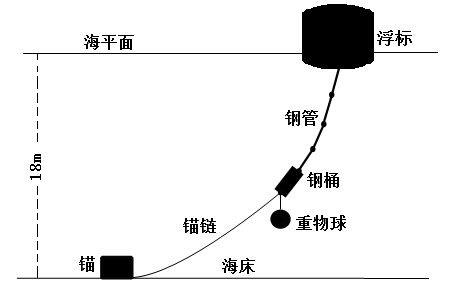
\includegraphics[width=0.8\textwidth]{img/title.jpg}
\caption{传输节点示意图(仅为结构模块示意图,未考虑尺寸比例)}\label{fig-buoy}
\end{figure}	

\begin{enumerate}[(1)]
	\item 

\end{enumerate}

\section{模型假设}
\begin{enumerate}
	\item

\end{enumerate}
\section{假设说明}
\begin{enumerate}
	\item 
	\item 
	
\end{enumerate}
\section{符号说明}
表\ref{table-symbol}列出了本文需要的符号。
\begin{table}[H]
	\centering
	\caption{符号说明} \label{table-symbol}
	\begin{tabular*}{\textwidth}{cc||cc}
		\hline
		符号 & 符号描述 & 符号 & 符号描述 \\
		\hline
		
		\hline
	\end{tabular*}
\end{table}

\section{问题分析}
\subsection{问题一的分析}
出库出库数据表中的数量主要受空调本身的属性、天气和经济数据影响。
而组织机构对空调销量的影响,主要就体现在天气与经济上。考虑到对于不同的地区,天气与经济的变化趋势均不相同,因此我们可以对每个组织机构分别训练通过时间预测
天气与经济的模型,再结合空调属性训练预测空调销量的模型。
\begin{figure}[H]
	\centering
	\includegraphics*[width=0.5\textwidth]{img_backup//q1_flowchart.png}
	\caption{问题一分析}
	\label{fig:q1_flowchart}
\end{figure}


\subsection{问题二的分析}


\subsection{问题三的分析}




\section{问题的解答}
\subsection{问题1的解答}
由于提供的数据中大量指标都是用中文描述,无法直接进行定量分析,因此需要将各个数据表中的数据进行量化与合并。
\subsubsection{数据的量化与处理}
\begin{enumerate}
	\item 天气指标的处理\par 
	在air\_temperature表中,需要量化的指标有天气现象,“风力风向”,
	“最高气温”与“最低气温”。首先处理天气现象列,将其中的各种天气按照恶劣程度从0至10编号,规则如表\ref{weather_quantify}所示。然后对每个单元格中的两个天气取平均值,
	得到一天的天气量化结果。
	\begin{table}[H]
		\centering
		\caption{天气量化方法} \label{weather_quantify}
		\begin{tabular*}{0.9\textwidth}{C{0.17\textwidth}C{0.17\textwidth}||C{0.23\textwidth}C{0.2\textwidth}}
			\hline
			天气名称 & 量化结果 & 天气名称 & 量化结果 \\
			\hline
			晴 & 0 & 小雨-中雨 & 4\\
			薄雾 & 0 &  小到中雨 & 4\\
			少云 & 0 & 雨夹雪 & 5\\
			晴间多云 & 0 & 沙尘暴 & 5\\
			阴 & 1 & 冻雨 & 5\\
			多云 & 1 & 中雨-大雨 & 5\\
			浮沙 & 1 & 中到大雨 & 5\\
			局部多云 & 1 & 雷阵雨 & 5\\
			刮风 & 1 & 暴雨 & 6\\
			小雨 & 2 & 大到暴雨 & 6 \\
			阵雨 & 2 & 小到中雪 & 7\\
			扬沙 & 2 & 暴雨到大暴雨 & 7 \\
			雾 & 2 & 中雪 & 8\\
			中度霾 & 2  & 中到大雪 & 8\\
			中雨 & 3 & 大暴雨到特大暴雨 & 8\\
			零散阵雨 & 3 & 雷阵雨伴有冰雹 & 8\\
			重度霾 & 3 & 大雪 & 9\\
			零散雷雨 & 4 & 大到暴雪 & 10\\
			雷阵雨 & 4 & & \\
			
			\hline
		\end{tabular*}
	\end{table}

	接着处理“风力风向”列。由于风向不易量化,因此仅提取出每个单元格中所有的风力大小,并求和取平均值。若单元格中没有风力大小,则用风力大小的平均值填充。
	最后处理“最高气温”与maxairtemperature列,先对最高温与最低温取平均值得到一天的平均气温,再对于数据缺失的单元格填充平均值。
	经过量化、删除无关指标“获取时间”、并且将时间指标改写为距2016年1月1日的天数后的air\_temperature表部分如下。
	\begin{table}[H]
		\centering
		\caption{处理后的air\_temperature表} \label{air_temperature_processed}
		\begin{tabular*}{\textwidth}{cccccccc}
			\hline
			date(天) & province & city & 天气现象 & 风力风向 & 最高气温($^{\circ}$C) & 最低气温($^{\circ}$C)\\
			\hline
			0 & 贵州 & 六盘水 & 4 & 4 & 6 & 4\\
			0 & 贵州 & 贵阳 & 3 & 3.333333333 & 10 & 6\\
			0 & 贵州 & 安顺 & 4 & 3.333333333 & 10 & 6\\
			0 & 贵州 & 遵义 & 3 & 3.5 & 12 & 6\\
			\hline
		\end{tabular*}
	\end{table}

	对数据进行量化处理后,就可以分析某一地点时间与各项天气指标的相关性,来确定使用哪些指标来代表天气。首先使用神经网络对四项天气指标关于时间的变化进行拟合,以重庆为例得到的结果如下。
	\begin{figure}[H]
		\begin{minipage}[t]{0.5\linewidth}
		  \centering   
		  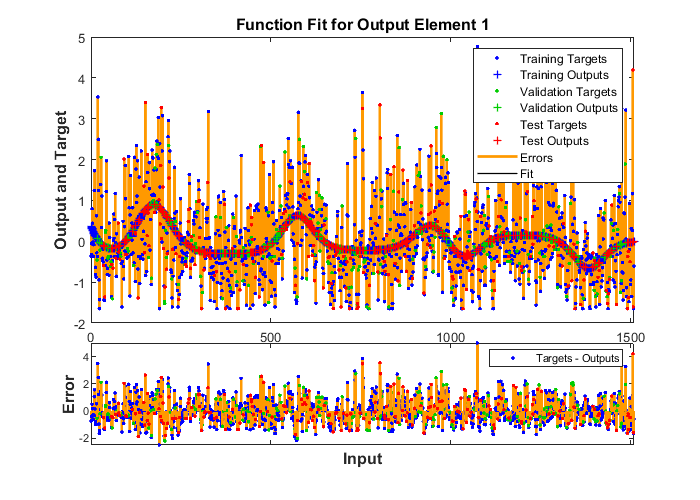
\includegraphics[width=0.95\textwidth]{img_backup/weather_fit.png}   
		  \caption{天气现象关于时间的拟合结果}   
		  \label{fig:weather_fit}   
		\end{minipage}   
		 \begin{minipage}[t]{0.5\linewidth} % 如果一行放2个图,用0.5,如果3个图,用0.33  
			\centering   
			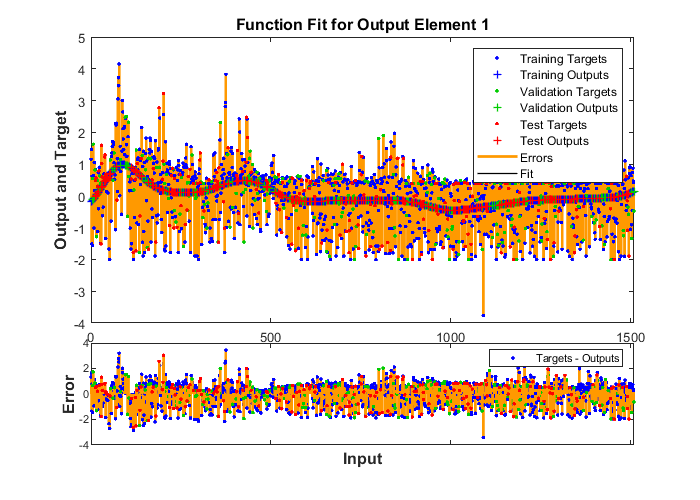
\includegraphics[width=0.95\textwidth]{img_backup/wind_fit.png}   
			\caption{“风力风向”关于时间的拟合结果}   
			\label{fig:wind_fit}   
		  \end{minipage} 
	  \end{figure}
	  \begin{figure}[H]
		  \centering   
		  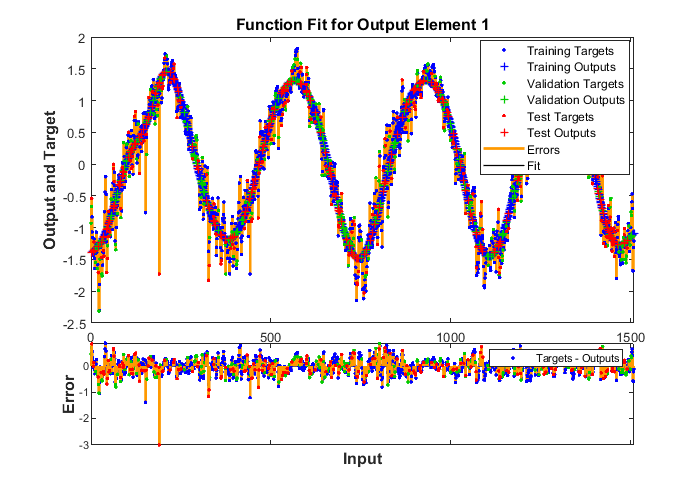
\includegraphics[width=0.8\textwidth]{img_backup/avetemp_fit.png}   
		  \caption{平均气温关于时间的拟合结果}   
		  \label{fig:avetemp_fit}   
	  \end{figure}
	  各项指标的方程确定系数$R$如表\ref{R_fit}所示。
	  \begin{table}[!htp]
		\centering
		\caption{各项指标的方程确定系数$R$} \label{R_fit}
		\centering
		\begin{tabular*}{0.55\textwidth}{ccc}
			\hline
			天气现象 & 风力风向 & 平均气温 \\
			\hline
			3.468 & 2.448 & 9.276 \\
			\hline
		\end{tabular*}
	\end{table}

	由于$R$越接近1代表拟合结果越准确,而天气现象与“风力风向”的拟合结果中$R$值均较低,因此
	可以认为天气现象与“风力风向”的变化与时间没有明显的相关性,而平均气温拟合的%因此在之后的预测中我们只使用平均气温这项指标来代表天气。
	\item 空调指标的量化\par 
	由于空调本身的性能也会影响空调销量,因此需要量化空调指标。由于许多指标并不能直接判断优劣,因此需要通过该指标与销量的关系确定
	\item 经济指标的处理\par 
	由于model\_stats\_new\_data表中除了全国的经济数据其他记录均有大量数据缺失,所以在筛选数据时只考虑全国经济数据。在各项指标中,由于“制造业固定资产投资额\_累计值”、
	“国有固定资产投资额\_累计值”、“建筑安装工程固定资产投资完成额\_累计值”、“综合PMI产出指数”这四项指标的数据有大量缺失,因此舍弃,其他缺失的数据用平均值填充。

	由于各项经济指标之间可能相互影响,因此使用主成分分析进行降维,得到结果如下。
	\begin{equation}
		\left[
\begin{array}{cccccc}
-0.0299 & -0.2834 & 0.2571 & 0.3842 & -0.3014 & 0.0083\\
0.0498 & 0.3054 & 0.1461 & -0.0301 & -0.3150 & 0.5692\\
-0.0754 & -0.3801 &	0.1526 & 0.3004 & -0.1140 & -0.1200\\
0.1968 & 0.2864 & -0.2604 & 0.2115 & -0.0242 & -0.0021\\
0.1968 & 0.2864 & -0.2604 & 0.2115 & -0.0242 & -0.0021\\
-0.2352 & 0.1885 & 0.0647 & -0.0523 & 0.1785 & 0.4359\\
-0.1448 & -0.1089 & 0.2108 & 0.1802 & 0.6028 & -0.0088\\
-0.0701 & 0.0834 & -0.2041 & 0.5533 & 0.1978 & 0.2196\\
0.1836 & -0.1261 & 0.1716 & 0.0946 & 0.3246 & 0.0477\\
0.1694 & 0.1306 & -0.4186 & 0.0320 & 0.0201 & -0.4219\\
0.3545 & -0.1473 & 0.1128 & -0.0520 & -0.0724 & 0.0476\\
0.3520 & -0.1527 & 0.1189 & -0.0581 & -0.0743 & 0.0471\\
0.3688 & -0.0768 & 0.0946 & -0.0247 & -0.0544 & 0.0924\\
0.3654 & -0.0999 & 0.0886 & -0.0826 & -0.0436 & 0.0195\\
0.2947 & -0.1357 & -0.1587 & 0.2702 & -0.0068 & 0.1535\\
0.3014 & -0.0202 & -0.0355 & 0.1519 & 0.3134 & 0.1820\\
0.2455 & 0.0934 & 0.1100 & -0.3800 & 0.3635 & 0.0099\\
0.0575 & 0.3527 & 0.3489 & 0.1547 & -0.0503 & -0.2412\\
0.0459 & 0.3127 & 0.3652 & 0.1426 & 0.0528 & -0.3336\\
0.0857 & 0.3463 & 0.3483 & 0.1490 & -0.0656 & -0.0579\\
\end{array}
\right]^\mathrm{ T }
\left[
\begin{array}{c}
    x_{1} \\
	x_{2} \\
	x_{3} \\
	x_{4} \\
	x_{5} \\
	x_{6} \\
	x_{7} \\
	x_{8} \\
	x_{9} \\
	x_{10} \\
	x_{11} \\
	x_{12} \\
	x_{13} \\
	x_{14} \\
	x_{15} \\
	x_{16} \\
	x_{17} \\
	x_{18} \\
	x_{19} \\
	x_{20} \\
\end{array}
\right]
=
\left[
\begin{array}{c}
    y_{1} \\
	y_{2} \\
	y_{3} \\
	y_{4} \\
	y_{5} \\
	y_{6} \\
\end{array}
\right]
\end{equation}
$y_i(i=1...6)$即为求得的6个主成分。
\end{enumerate}
 
\subsubsection{指标分析}
\begin{enumerate}
	\item 天气指标的分析\par
	作销量和平均气温关于时间的折线图如下
	\begin{figure}[H]
		\centering
		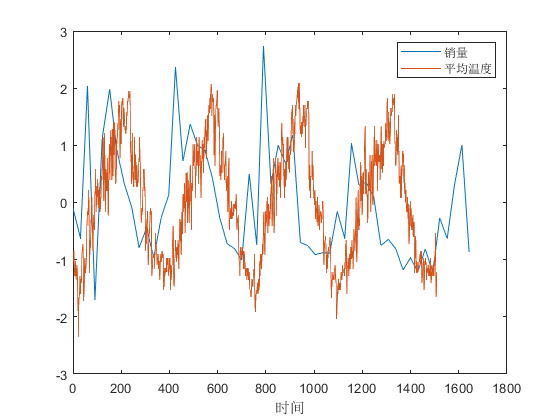
\includegraphics[width=0.95\textwidth]{img_backup/temp-sales.png}   
		\caption{销量和平均气温随时间的变化图}  \label{fig:temp_sales}
	\end{figure}
	从图\ref{fig:temp_sales}中可以看出,空调销量与平均气温都呈周期性变化,周期约为一年,且空调销量的变化要晚于平均气温的变化。
	\item 经济指标的分析\par
	对6个主成分分别作其和空调销量关于时间的折线图
	\begin{figure}[H]
		\begin{minipage}[t]{0.5\linewidth}   
		  \centering   
		  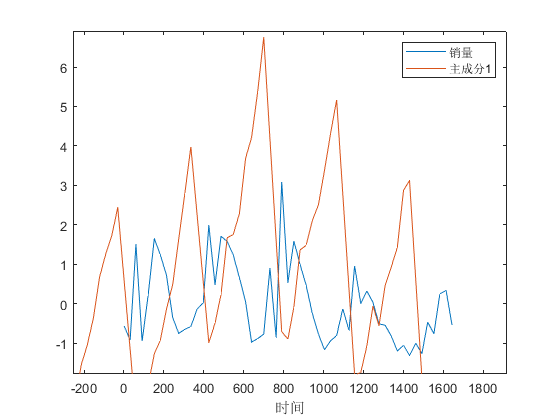
\includegraphics[width=0.8\textwidth]{img_backup/pca1-sales.png}   
		  \caption{销量和$y_1$随时间的变化图}   
		  \label{fig:pca1_sales}   
		\end{minipage}   
		 \begin{minipage}[t]{0.5\linewidth} % 如果一行放2个图,用0.5,如果3个图,用0.33  
			\centering   
			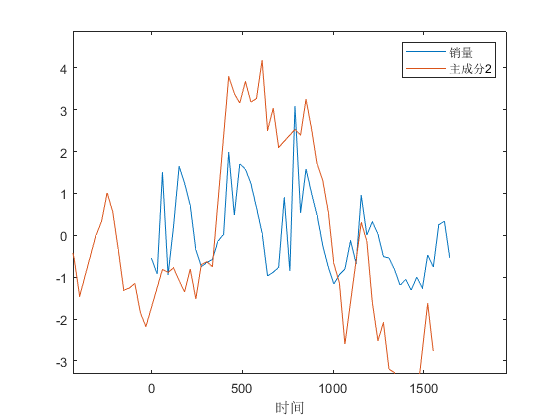
\includegraphics[width=0.8\textwidth]{img_backup/pca2-sales.png}   
			\caption{销量和$y_2$随时间的变化图}   
			\label{fig:pca2_sales.png}
		  \end{minipage} 
	  \end{figure}
	  \begin{figure}[H]
		\begin{minipage}[t]{0.5\linewidth}   
		  \centering   
		  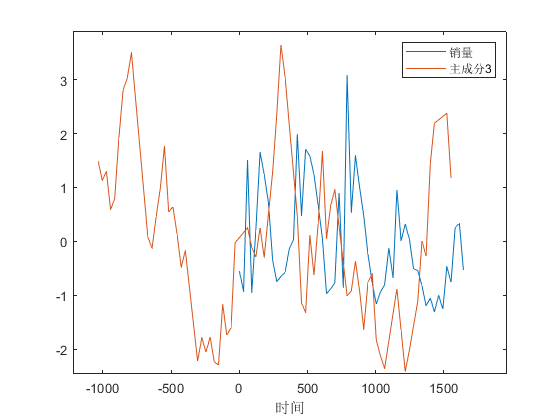
\includegraphics[width=0.8\textwidth]{img_backup/pca3-sales.png}   
		  \caption{销量和$y_3$随时间的变化图}   
		  \label{fig:pca3_sales}   
		\end{minipage}   
		 \begin{minipage}[t]{0.5\linewidth} % 如果一行放2个图,用0.5,如果3个图,用0.33  
			\centering   
			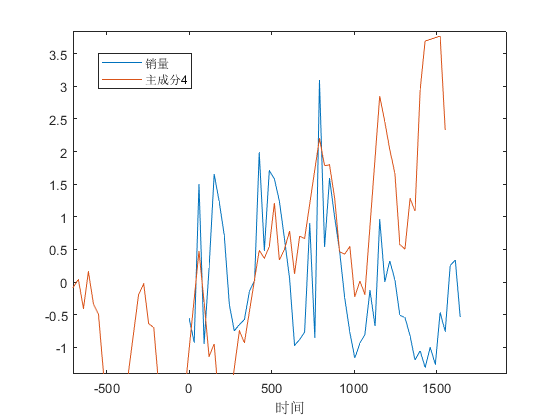
\includegraphics[width=0.8\textwidth]{img_backup/pca4-sales.png}   
			\caption{销量和$y_4$随时间的变化图}   
			\label{fig:pca4_sales}   
		  \end{minipage} 
	  \end{figure}
	  \begin{figure}[H]
		\begin{minipage}[t]{0.5\linewidth}   
		  \centering   
		  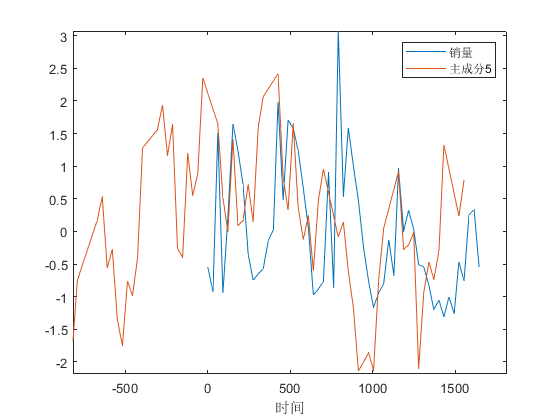
\includegraphics[width=0.8\textwidth]{img_backup/pca5-sales.png}   
		  \caption{销量和$y_5$随时间的变化图}   
		  \label{fig:pca5_sales}   
		\end{minipage}   
		 \begin{minipage}[t]{0.5\linewidth} % 如果一行放2个图,用0.5,如果3个图,用0.33  
			\centering   
			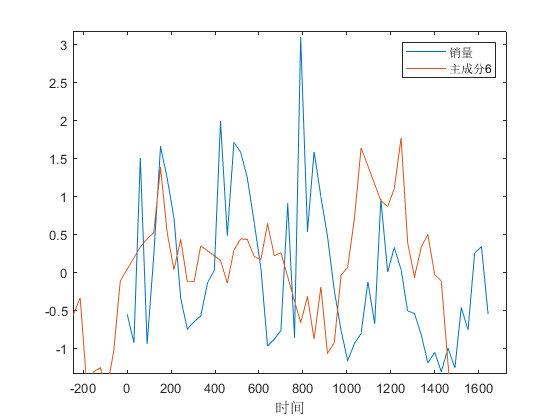
\includegraphics[width=0.8\textwidth]{img_backup/pca6-sales.png}   
			\caption{销量和$y_6$随时间的变化图}   
			\label{fig:pca6_sales}   
		  \end{minipage} 
	  \end{figure}
	从上图可以看出6个主成分与空调销量没有明显的联系,还需要进行进一步的分析。
\end{enumerate}

\subsubsection{销量预测}

\subsection{问题2的解答}
在问题一的假设下,将海面风速为36m/s时的各项计算结果如表\ref{table:result_2}和表\ref{table:pipe_angle_2},锚链形状如图\ref{fig:chain_shape_36}。
\begin{table}[!htp]
	\centering
	\caption{问题二部分计算结果}\label{table:result_2}
	\centering
	\begin{tabular*}{\textwidth}{ccccc}
		
		\hline
		风速$(m/s)$ & 钢桶倾斜角$(^\circ)$ & 吃水深度$(m)$ & 游动半径$(m)$ & 锚链参数$a$\\
		\hline
		36 & 8.0708 & 0.7700 & 18.7156  & 29.0460\\
		\hline
	\end{tabular*}
\end{table}
\begin{figure}[H]
	\centering
	\includegraphics*[width=0.5\textwidth]{img/36mschainfigure.jpg}
	\caption{风速为36$m/s$时的锚链形状}
	\label{fig:chain_shape_36}
\end{figure}
\begin{table}[H]
	\centering
	\caption{问题二钢管倾斜角计算结果}
	\label{table:pipe_angle_2}
	\begin{tabular*}{0.85\textwidth}{ccccc}
		\hline
		风速$(m/s)$ & 钢桶倾斜角1 & 钢桶倾斜角2 & 钢桶倾斜角3 & 钢桶倾斜角4\\
		\hline
		36 & 7.8454 & 7.8876 & 7.9302 & 7.9733\\
		\hline
	\end{tabular*}
\end{table}

由之前问题2的分析,我们的目标在于寻找重球重力的最小值,使得重球重力大于这个最小值时满足$\theta$和$\beta$的限制条件。\par
求$G_s$
\begin{displaymath}
	s.t.\left\{
	\begin{aligned}
	\theta\le 5^\circ\\
	\beta \le 16^\circ\\
	\end{aligned}
	\right.
\end{displaymath}
通过定长搜索得到$\theta$和$\beta$随$G_s$的变化趋势如图\ref{fig:theta_G_s}和图\ref{fig:beta_G_s}:
\begin{figure}[H]
  \begin{minipage}[t]{0.5\linewidth}   
    \centering
    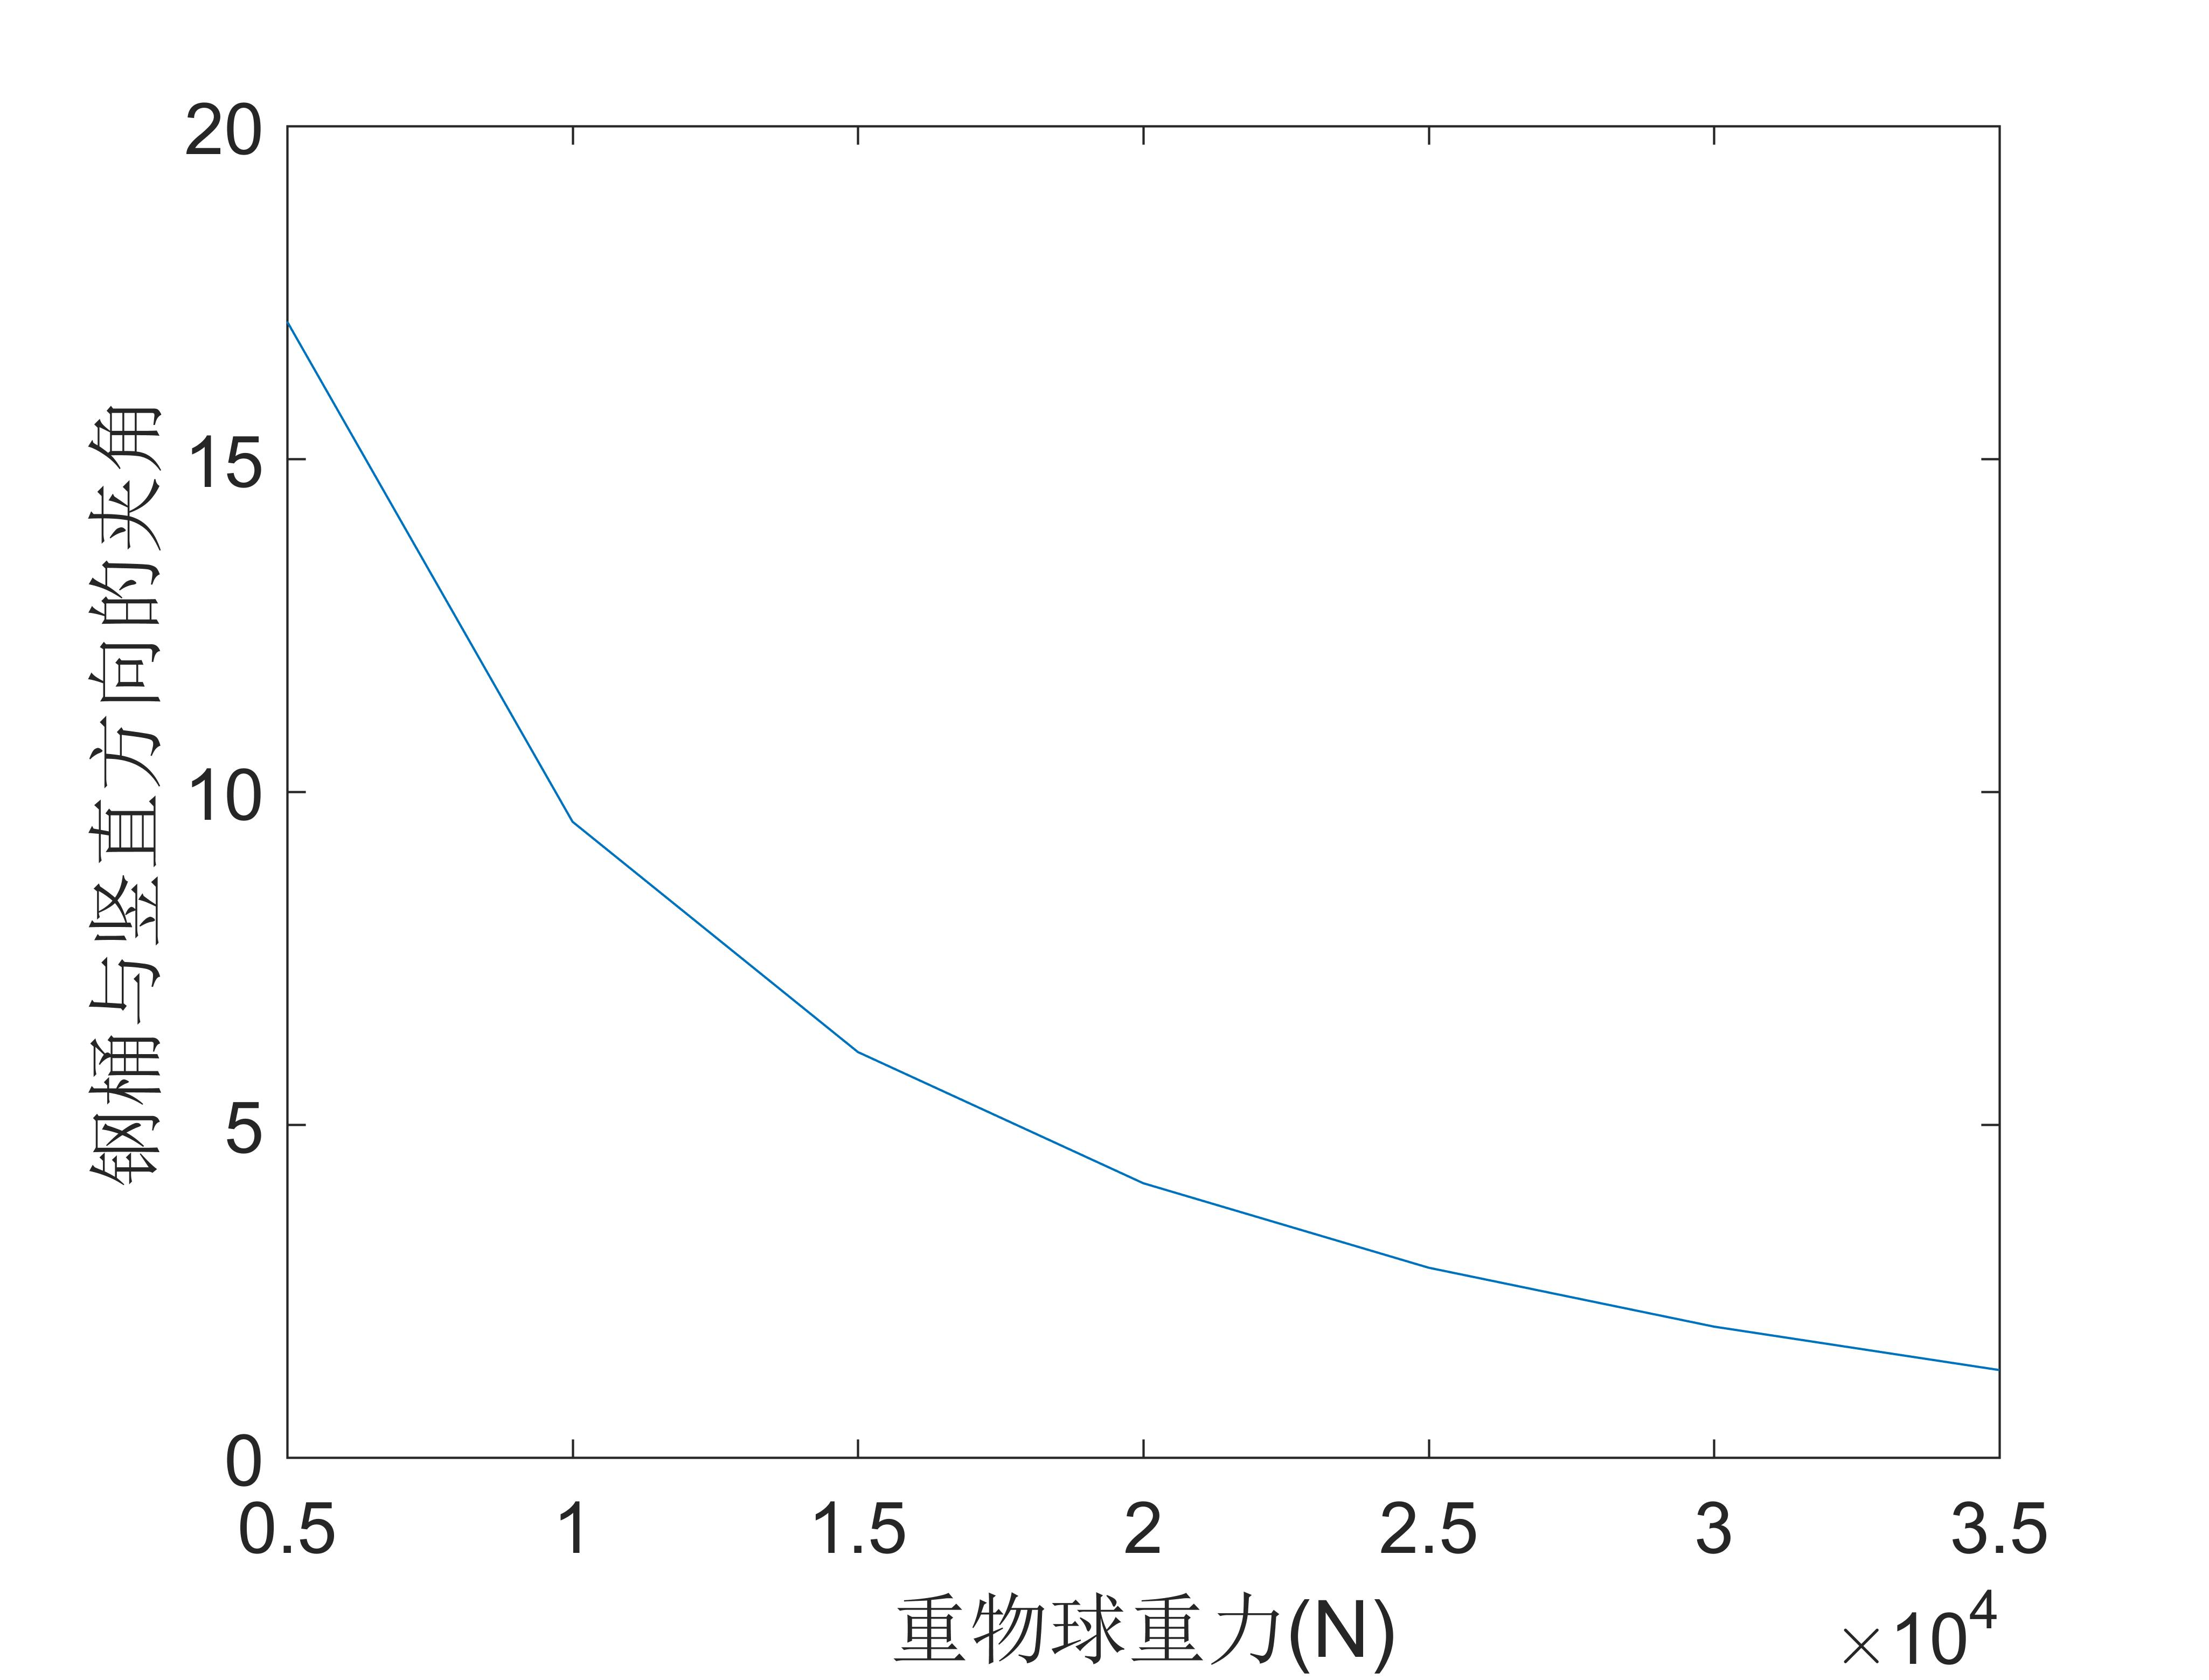
\includegraphics[width=\textwidth]{img/theta_G_s.jpg}   
    \caption{$\theta$随$G_s$变化曲线}   
    \label{fig:theta_G_s}   
  \end{minipage}
   \begin{minipage}[t]{0.5\linewidth} % 如果一行放2个图,用0.5,如果3个图,用0.33  
      \centering   
      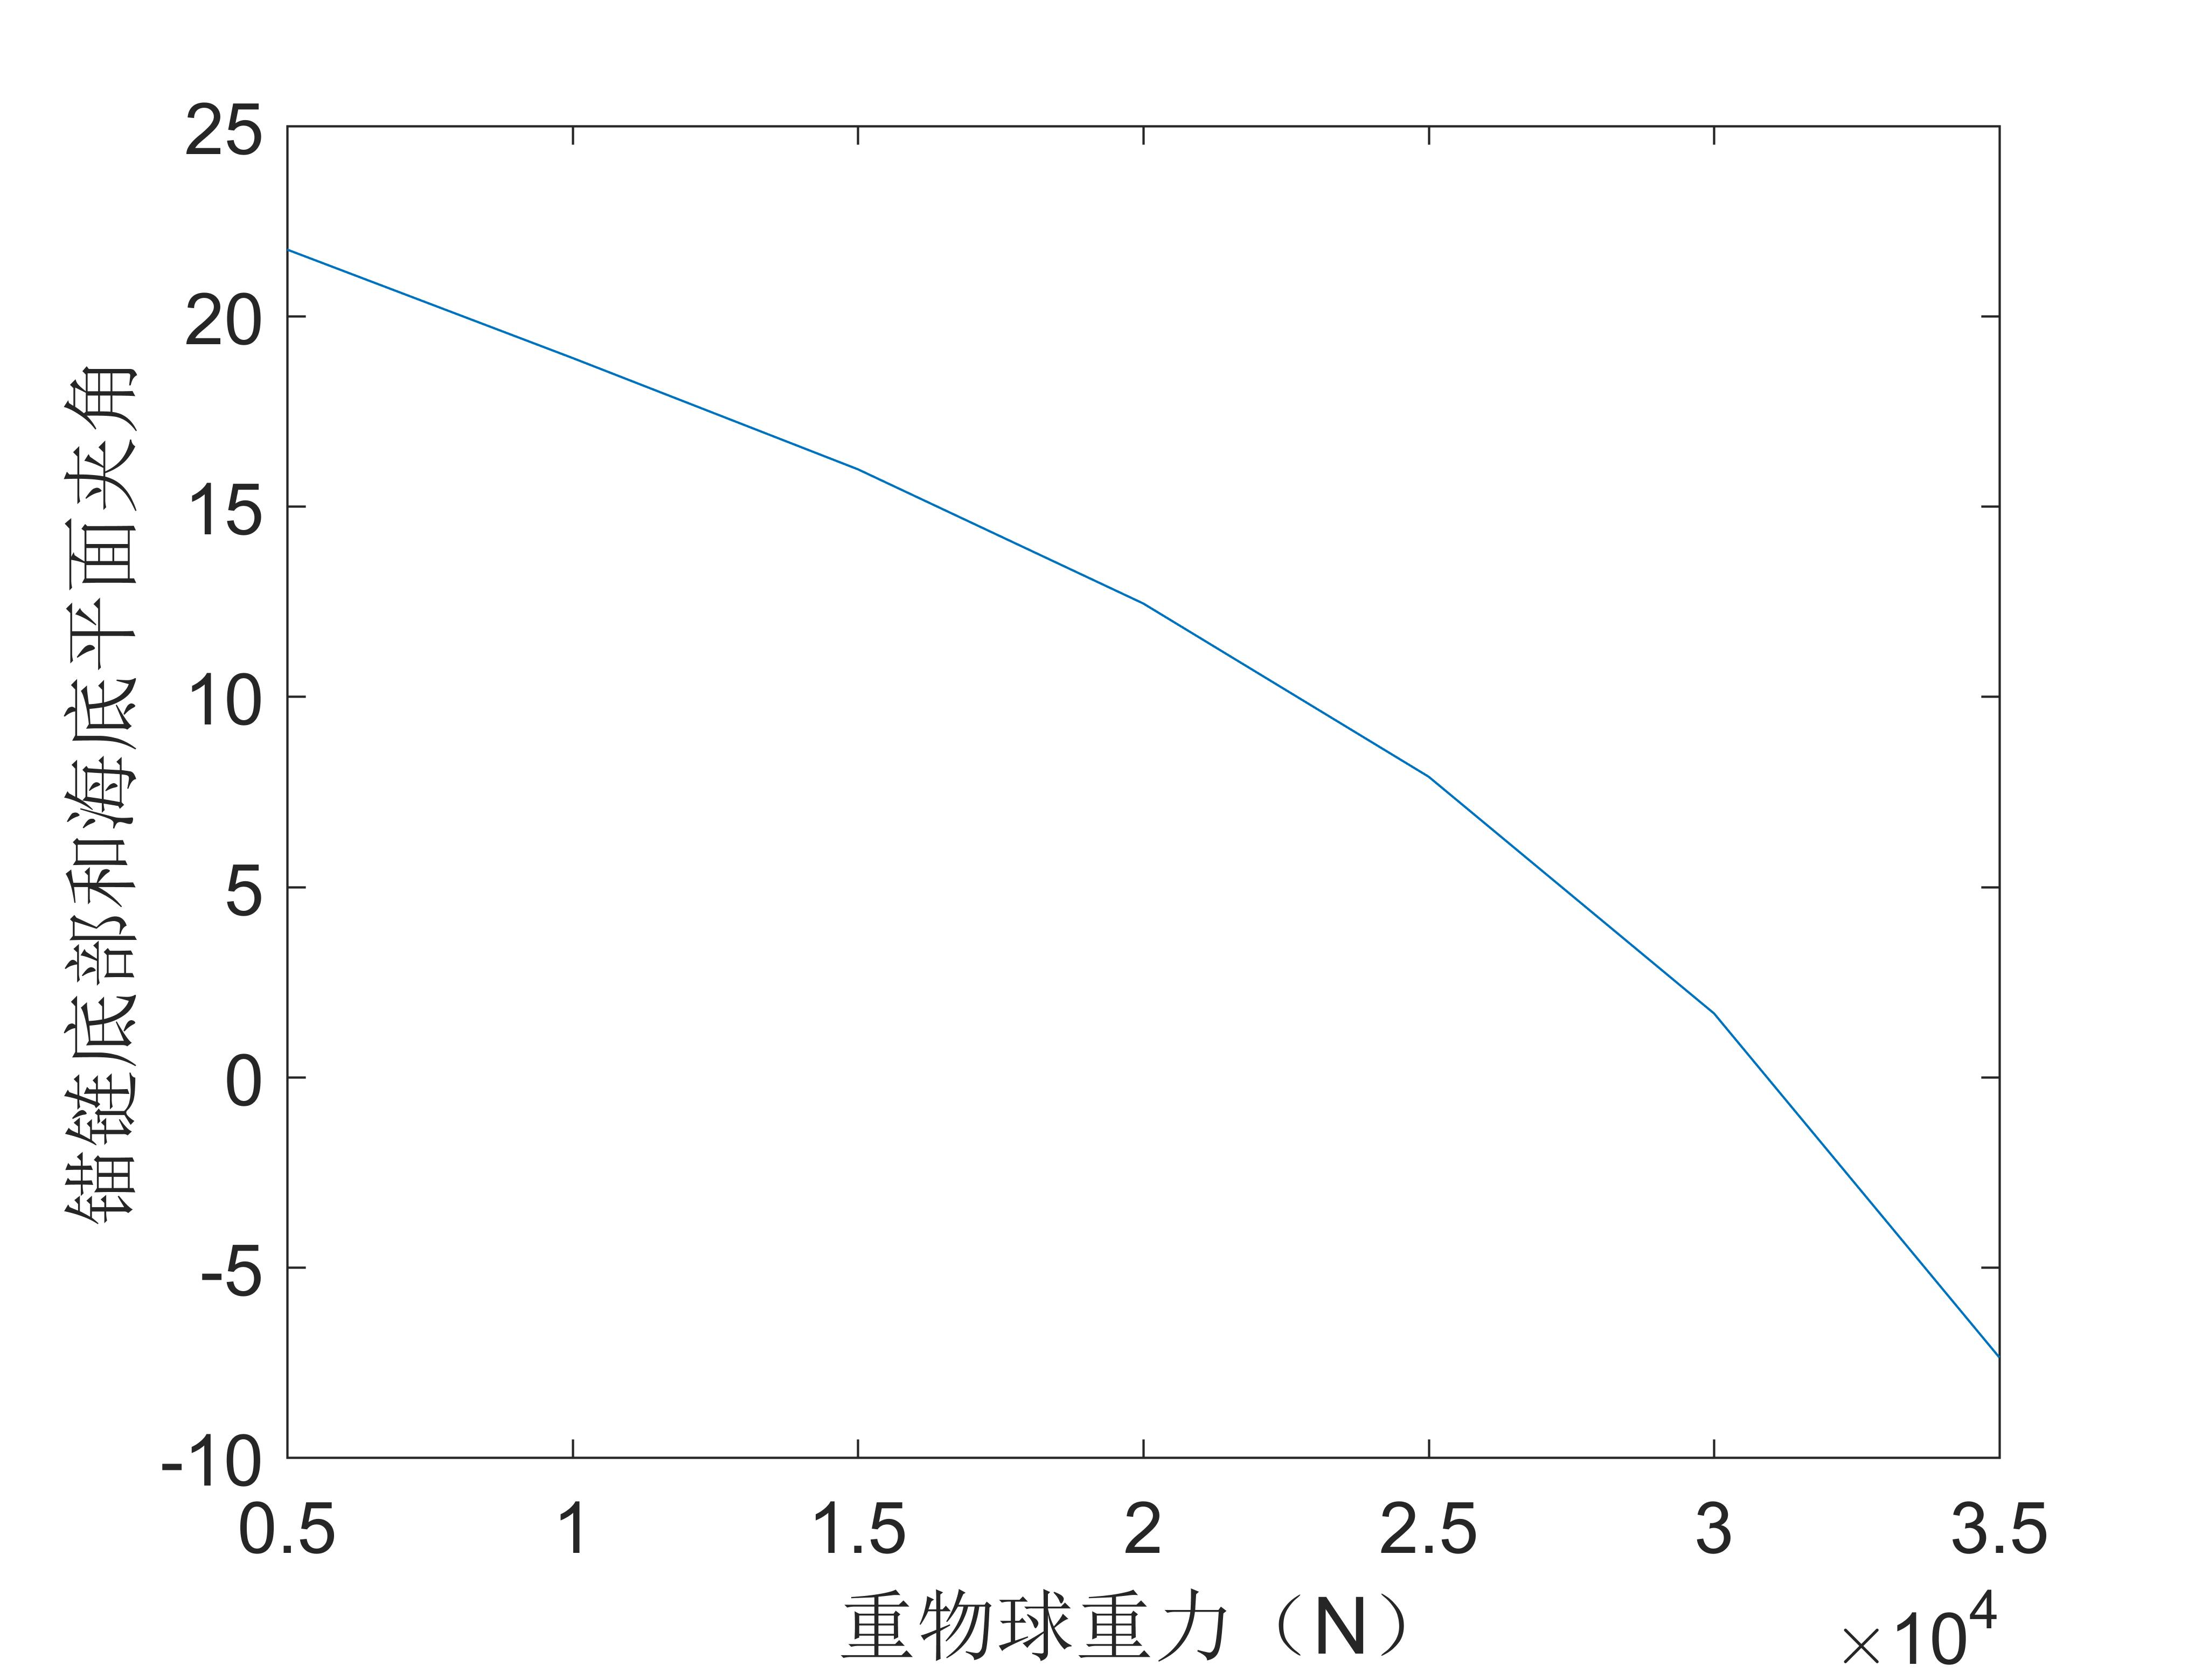
\includegraphics[width=\textwidth]{img/beta_G_s.jpg}   
      \caption{$\beta$随$G_s$变化曲线}   
      \label{fig:beta_G_s}   
    \end{minipage} 
\end{figure}
可以看到两者均为单调函数,故只有一个下限和上限,并可用二分法加快求解,算法如算法\ref{bs}:\par
\renewcommand{\algorithmicrequire}{\textbf{Input:}} 
\renewcommand{\algorithmicensure}{\textbf{Output:}}
\begin{algorithm} [H] 
	\caption{Binary search} %算法的题目 
	\label{bs} %算法的标签 
	\begin{algorithmic}[1] %此处的[1]控制一下算法中的每句前面都有标号 
		\REQUIRE {Upperbound left,lowerbound right and error restrictions $0.01$}
		\ENSURE{The weight of the ball}
		\WHILE{$|right-left|\geq0.01 \;\mathbf{and}\; angle(x_0)\neq5$}
		\IF {$angle(x_0)>5$}
		\STATE $left\leftarrow x_0$
		\ELSE
		\STATE $right\leftarrow x_0$
		\ENDIF
		\STATE $X_0\leftarrow(left+right)/2$
		\ENDWHILE
	\end{algorithmic} 
\end{algorithm}
根据图\ref{fig:theta_G_s}和图\ref{fig:beta_G_s}可对下限与上限进行二分法搜索,搜索结果为重物球质量的范围[1746.58,3172.29](单位:$kg$)。


\subsection{问题三的解答}
题目描述中,海水速度最大为$1.5m/s$,风速最大为$36m/s$。为简化模型,我们取海水速度以及风力速度均为最大值。我们将风速海速称为\textbf{环境恶劣程度}。将浮标、四节钢管看成一个整体,从直观上来看当环境越恶劣,即风速和水速越大时,这个整体受到钢桶的水平力$T_{5x}$越大,而$T_{5x}$对钢桶的力矩为顺时针转动,使得$\theta$越大,从问题一二的结果也可以验证这个猜想。故如果系泊系统在最恶劣环境下能够满足工作要求,那么系统肯定能够在平稳的环境中正常运行。\par
为了模型的建立,我们做了如下简化:
\begin{enumerate}
	\item 通过计算,水流对钢桶的力最大为$252N$,对钢管的力最大为$42N$,相对于拉力大小可以忽略不计。
	\item
	我们将水深16$m\sim 20m$的连续范围其离散化为三组$16m,18m,20m$分别进行计算。
\end{enumerate}\par 
首先我们尝试用锚链型号\uppercase\expandafter{\romannumeral2}和水深$18m$进行模型计算。由于限定了水深风速,对向量\\$(L,G_s)$($L$表示锚链长度,$G_s$表示重球质量)可以唯一确定一个系泊系统状态。我们在一定合理范围内遍历$(L,G_s)$,对钢桶倾斜角$\theta$、锚链底端切线与水平面夹角$\beta$、浮标露出水面高度$h$、浮标游动范围半径$distance$求值并作三维图像,如图\ref{fig:2_18_theta}、图\ref{fig:2_18_beta}、图\ref{fig:2_18_h}和图\ref{fig:2_18_distance}。
\begin{figure}[H]
  \begin{minipage}[t]{0.5\linewidth}   
    \centering   
    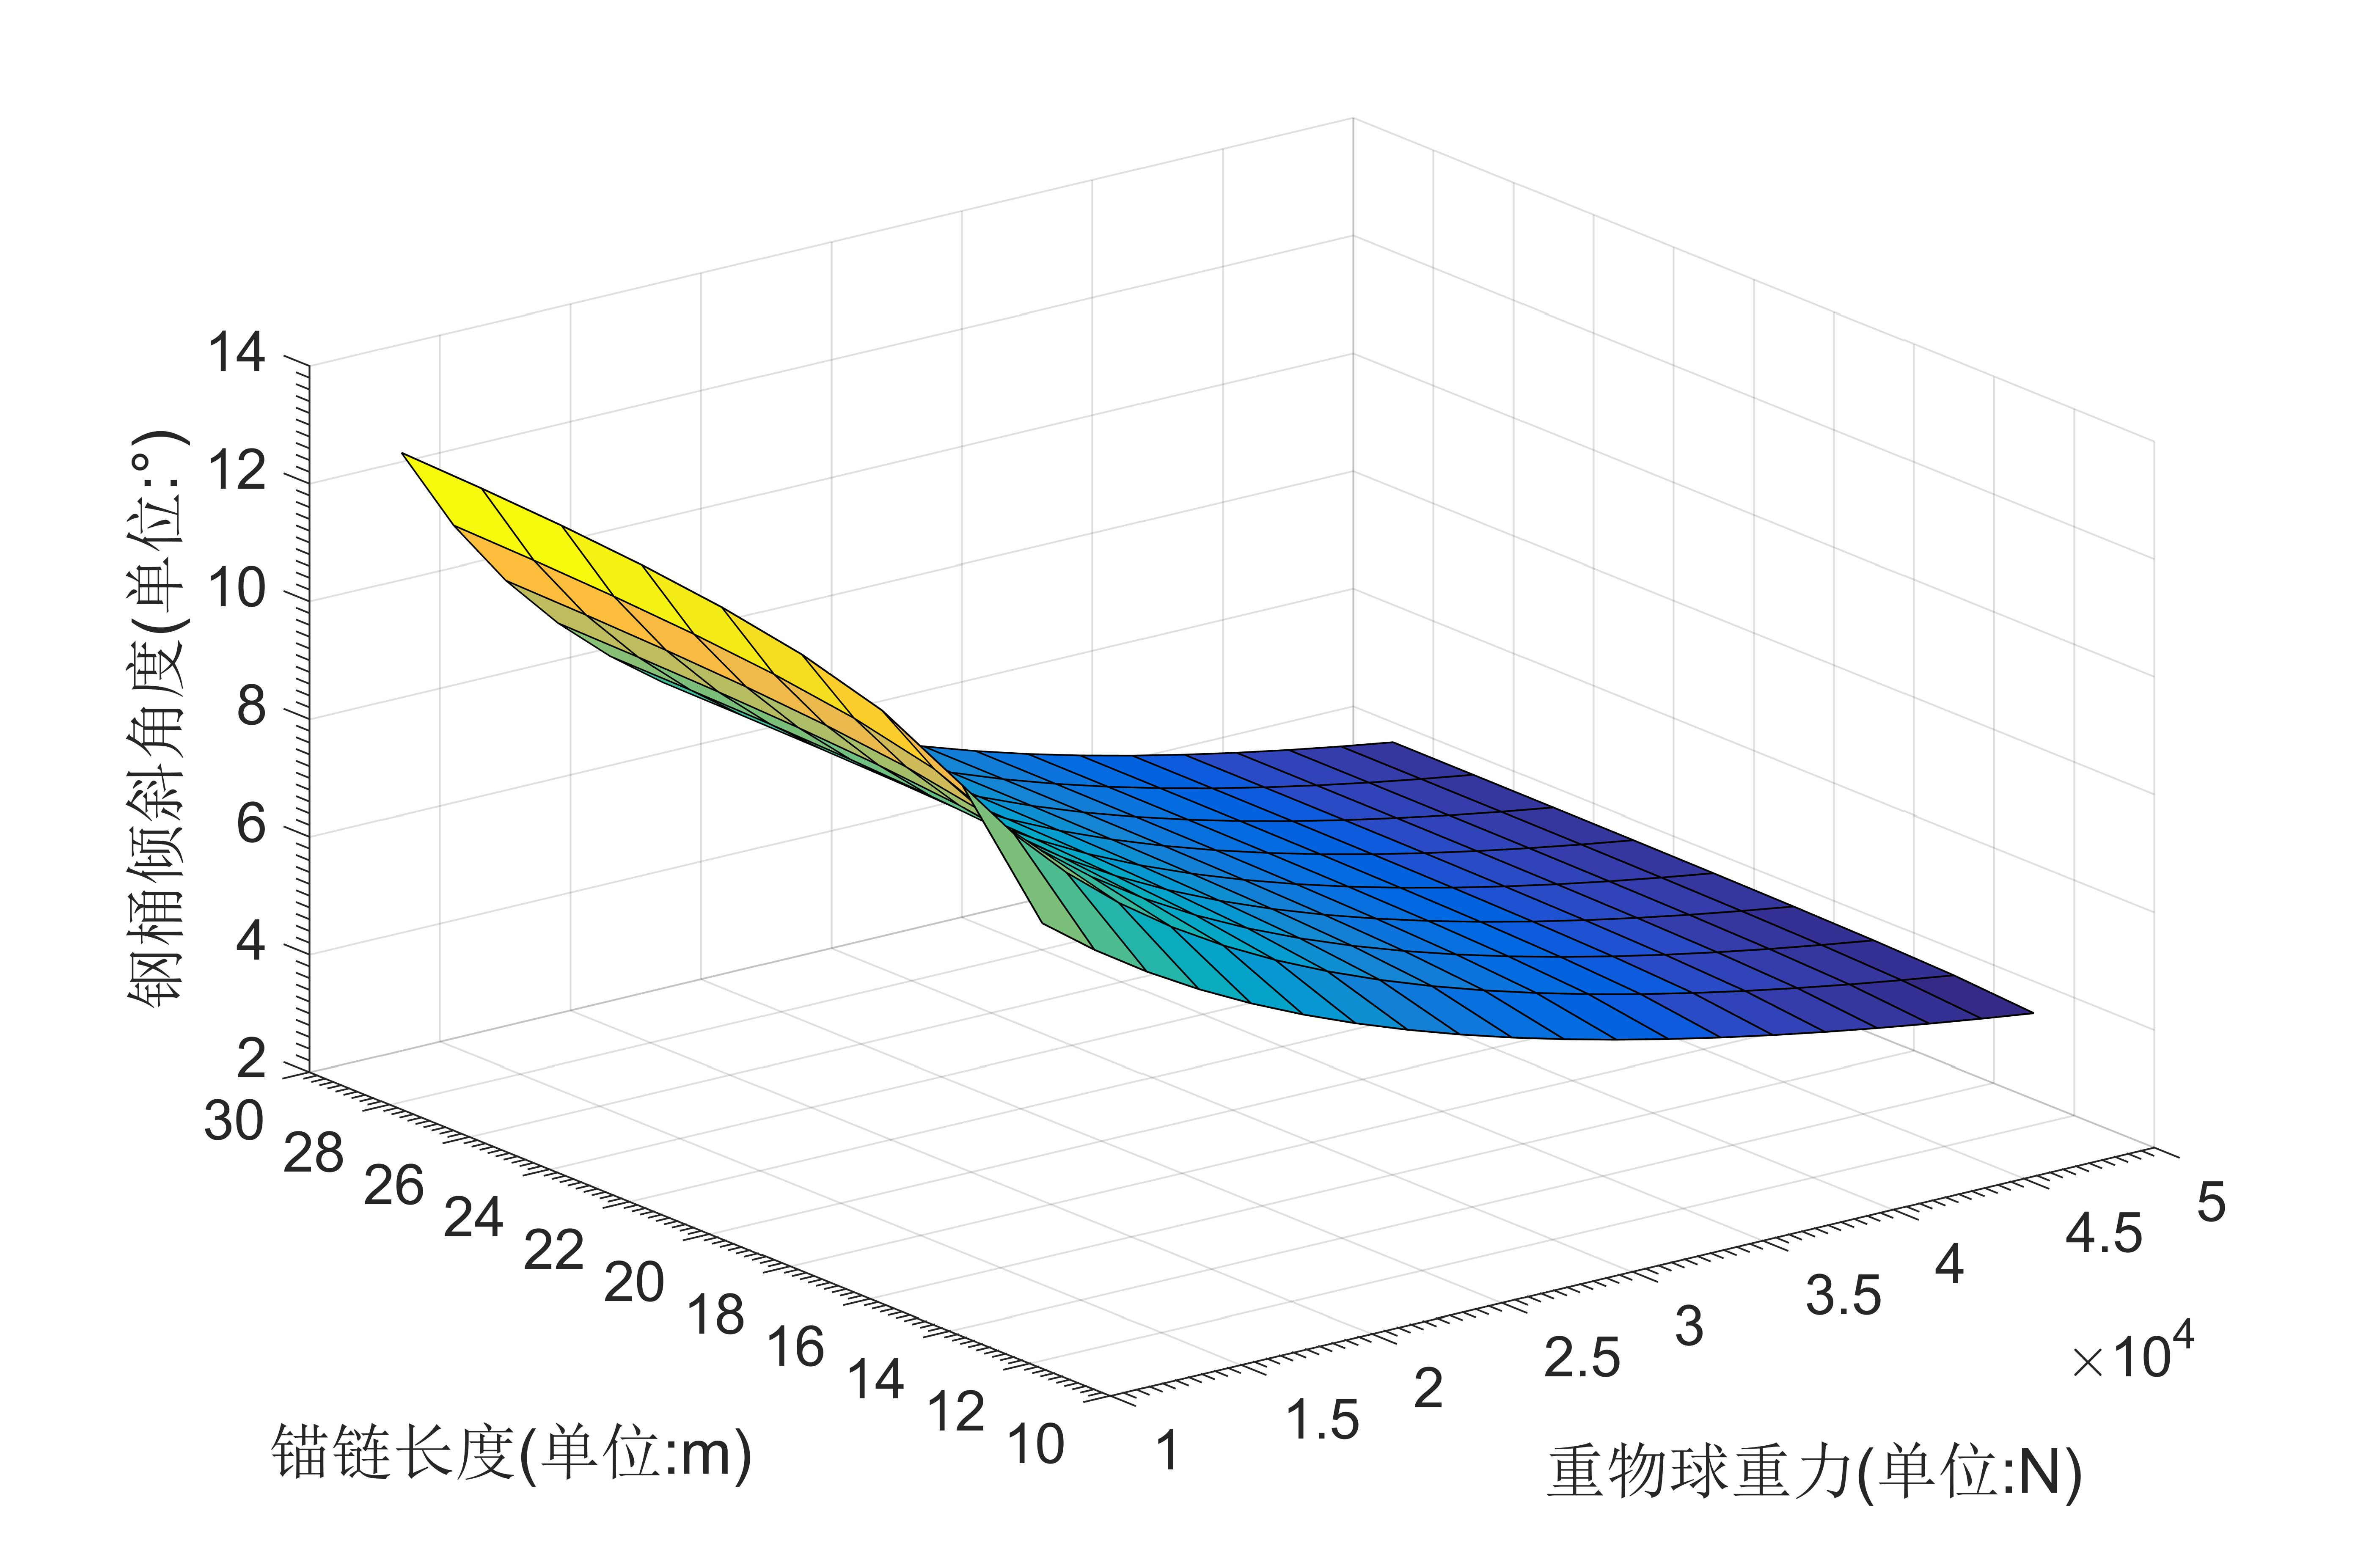
\includegraphics[width=\textwidth]{img/II_18_theta.jpg}   
    \caption{$\theta$变化图}   
    \label{fig:2_18_theta}   
  \end{minipage}
   \begin{minipage}[t]{0.5\linewidth} % 如果一行放2个图,用0.5,如果3个图,用0.33  
      \centering   
      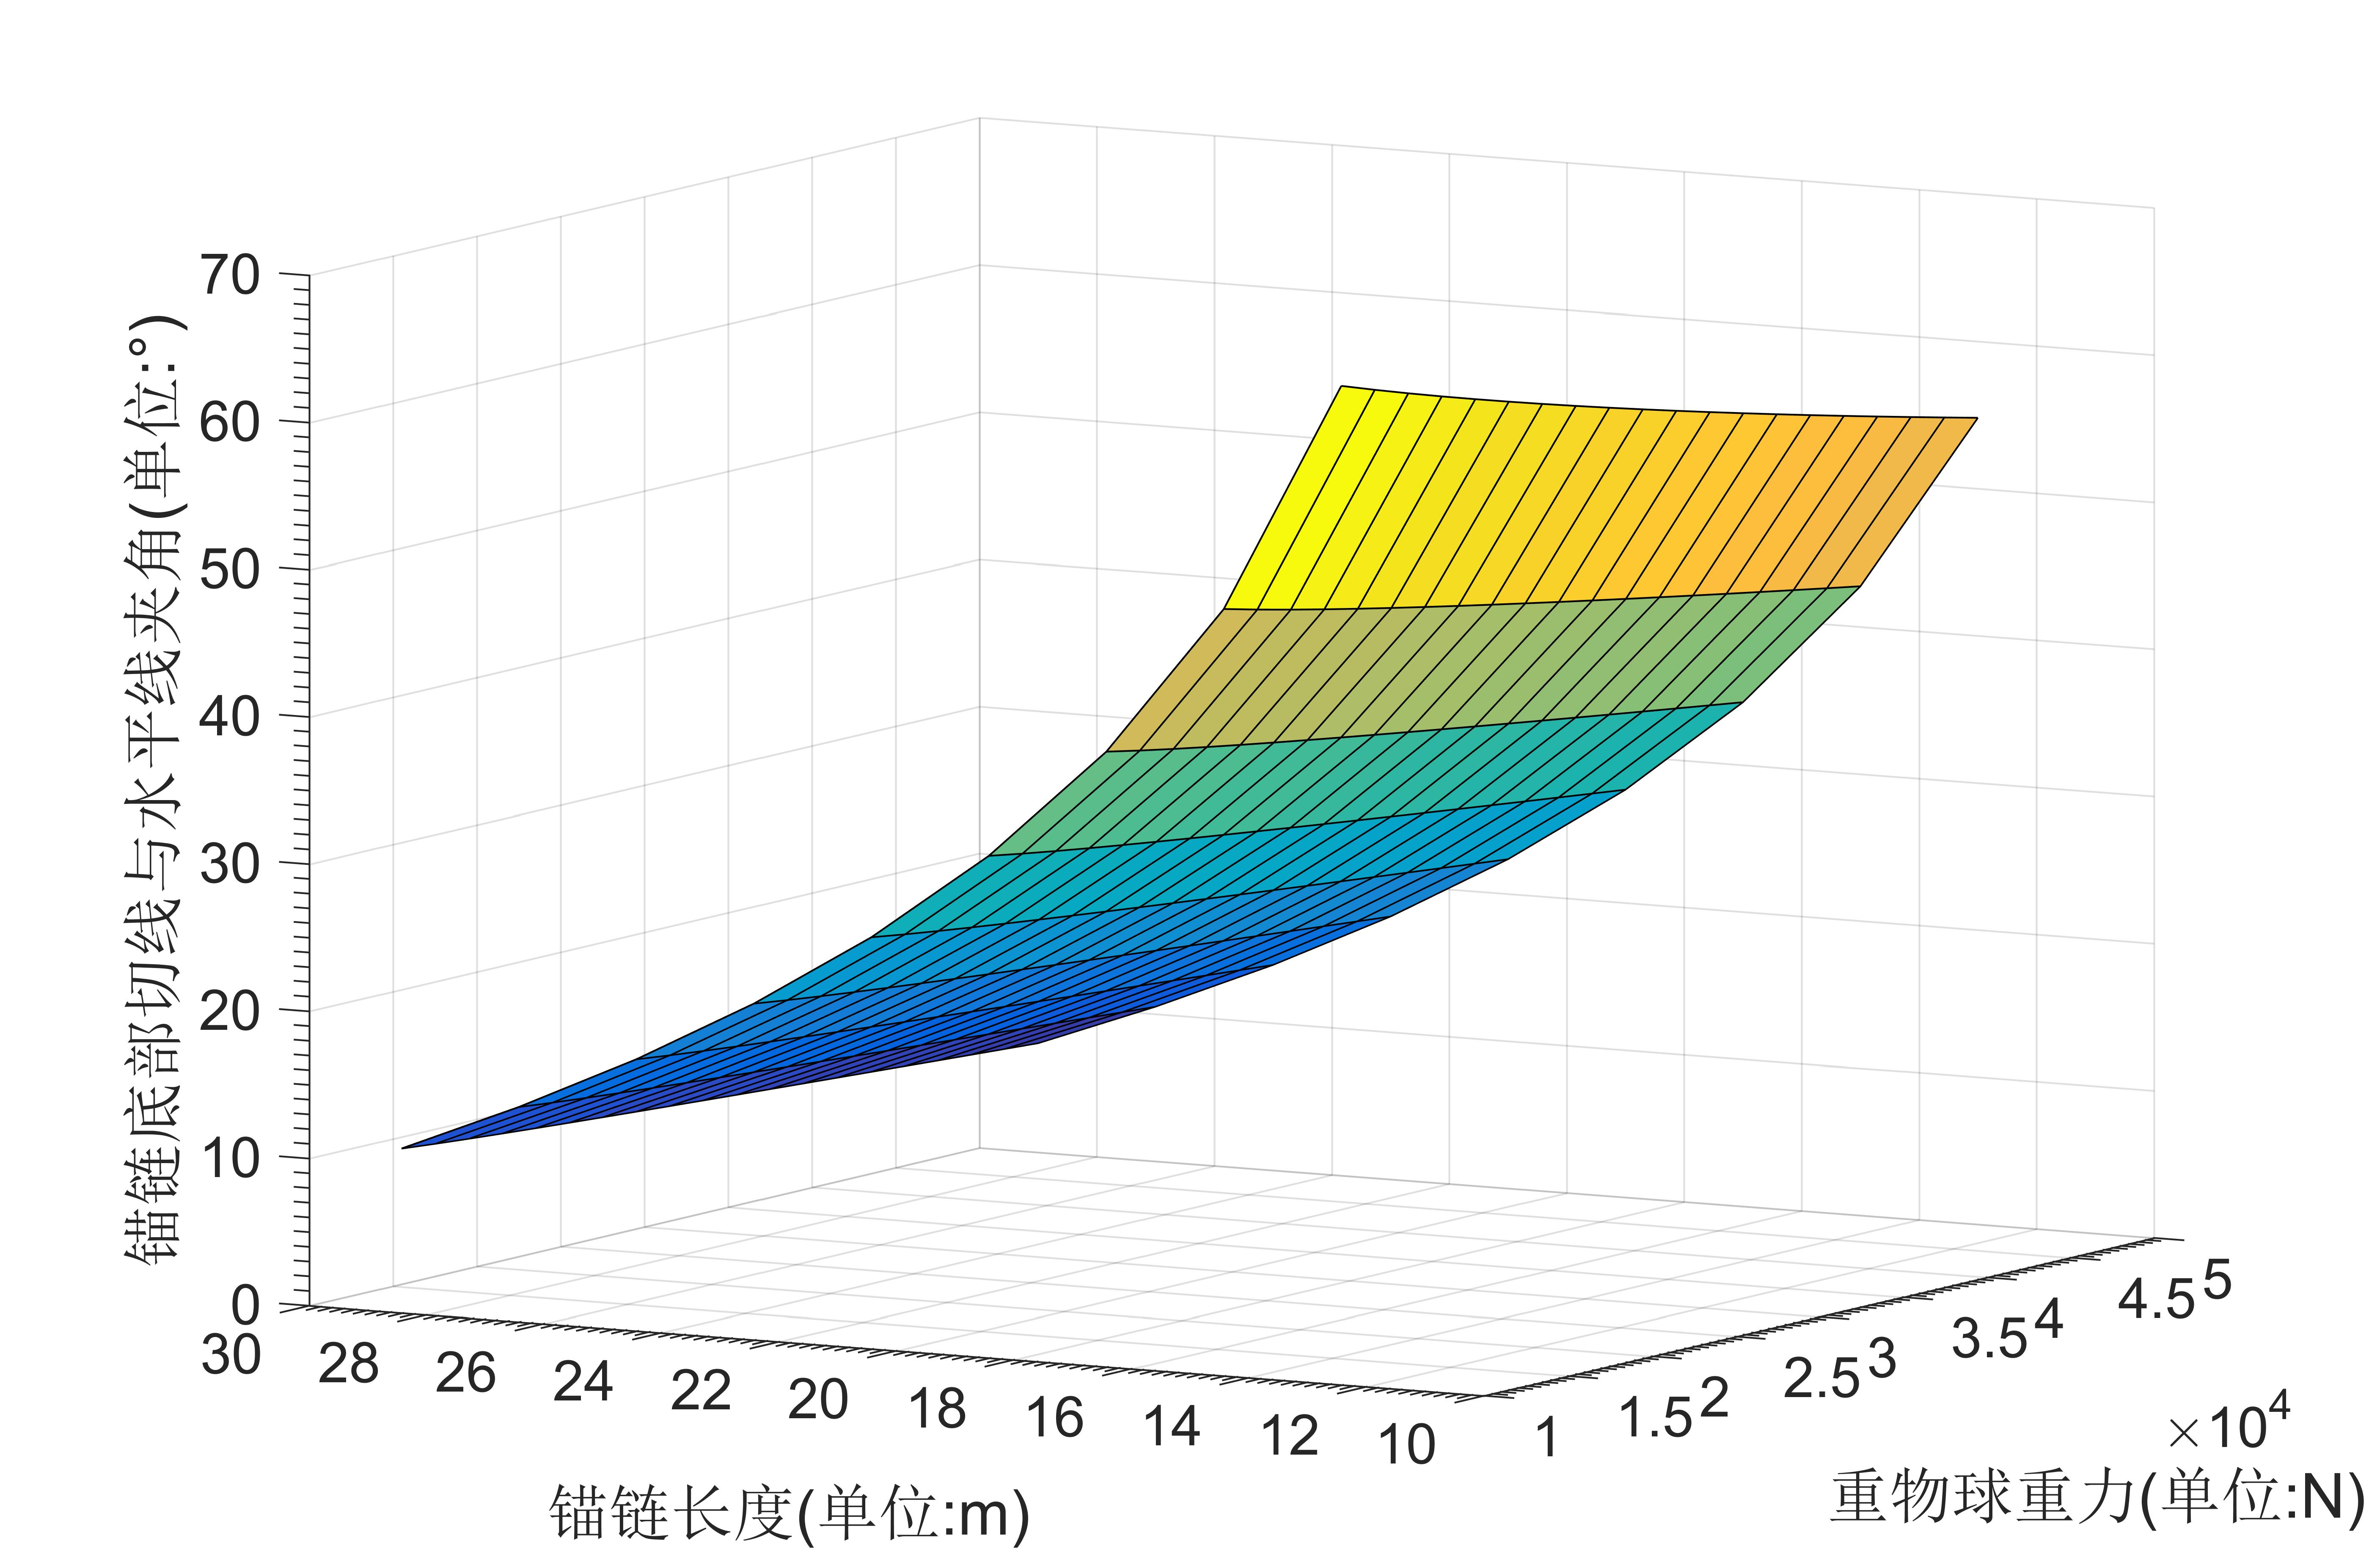
\includegraphics[width=\textwidth]{img/II_18_beta.jpg}   
      \caption{$\beta$变化图}   
      \label{fig:2_18_beta}   
    \end{minipage} 
\end{figure}
\begin{figure}[H]
  \begin{minipage}[t]{0.5\linewidth}   
    \centering   
    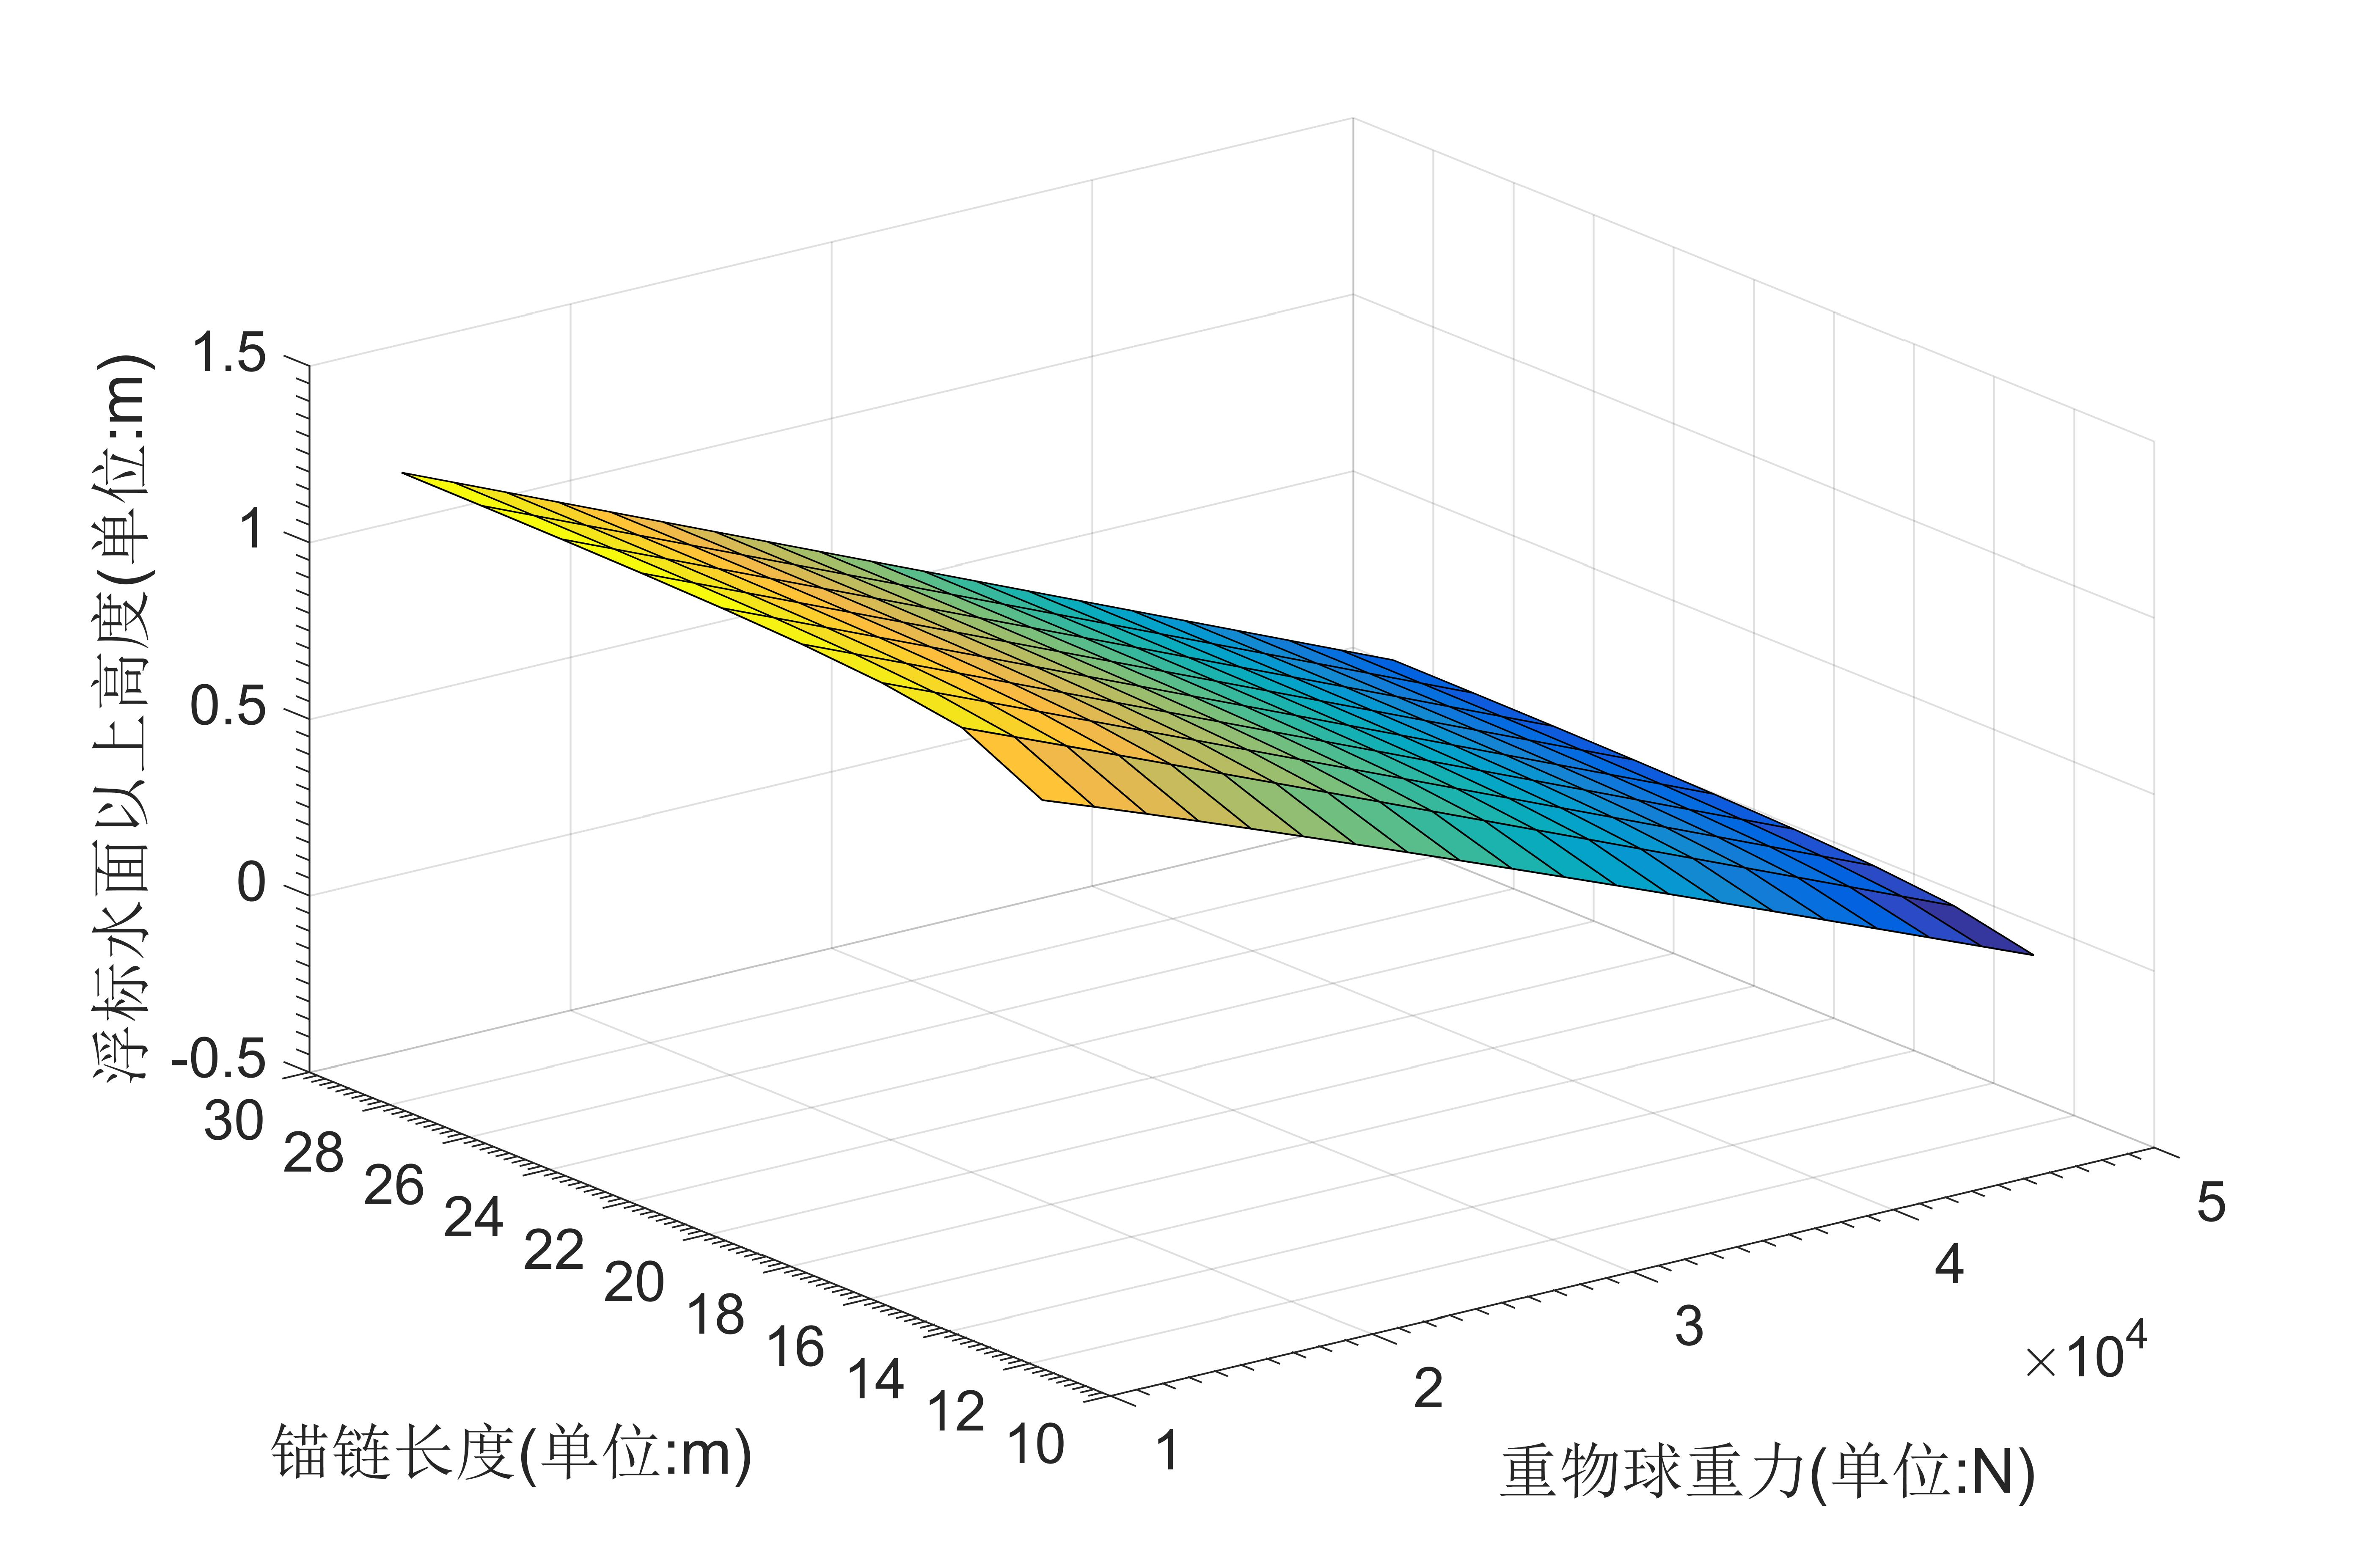
\includegraphics[width=\textwidth]{img/II_18_h.jpg}   
    \caption{$h$变化图}   
    \label{fig:2_18_h}   
  \end{minipage}
   \begin{minipage}[t]{0.5\linewidth} % 如果一行放2个图,用0.5,如果3个图,用0.33  
      \centering   
      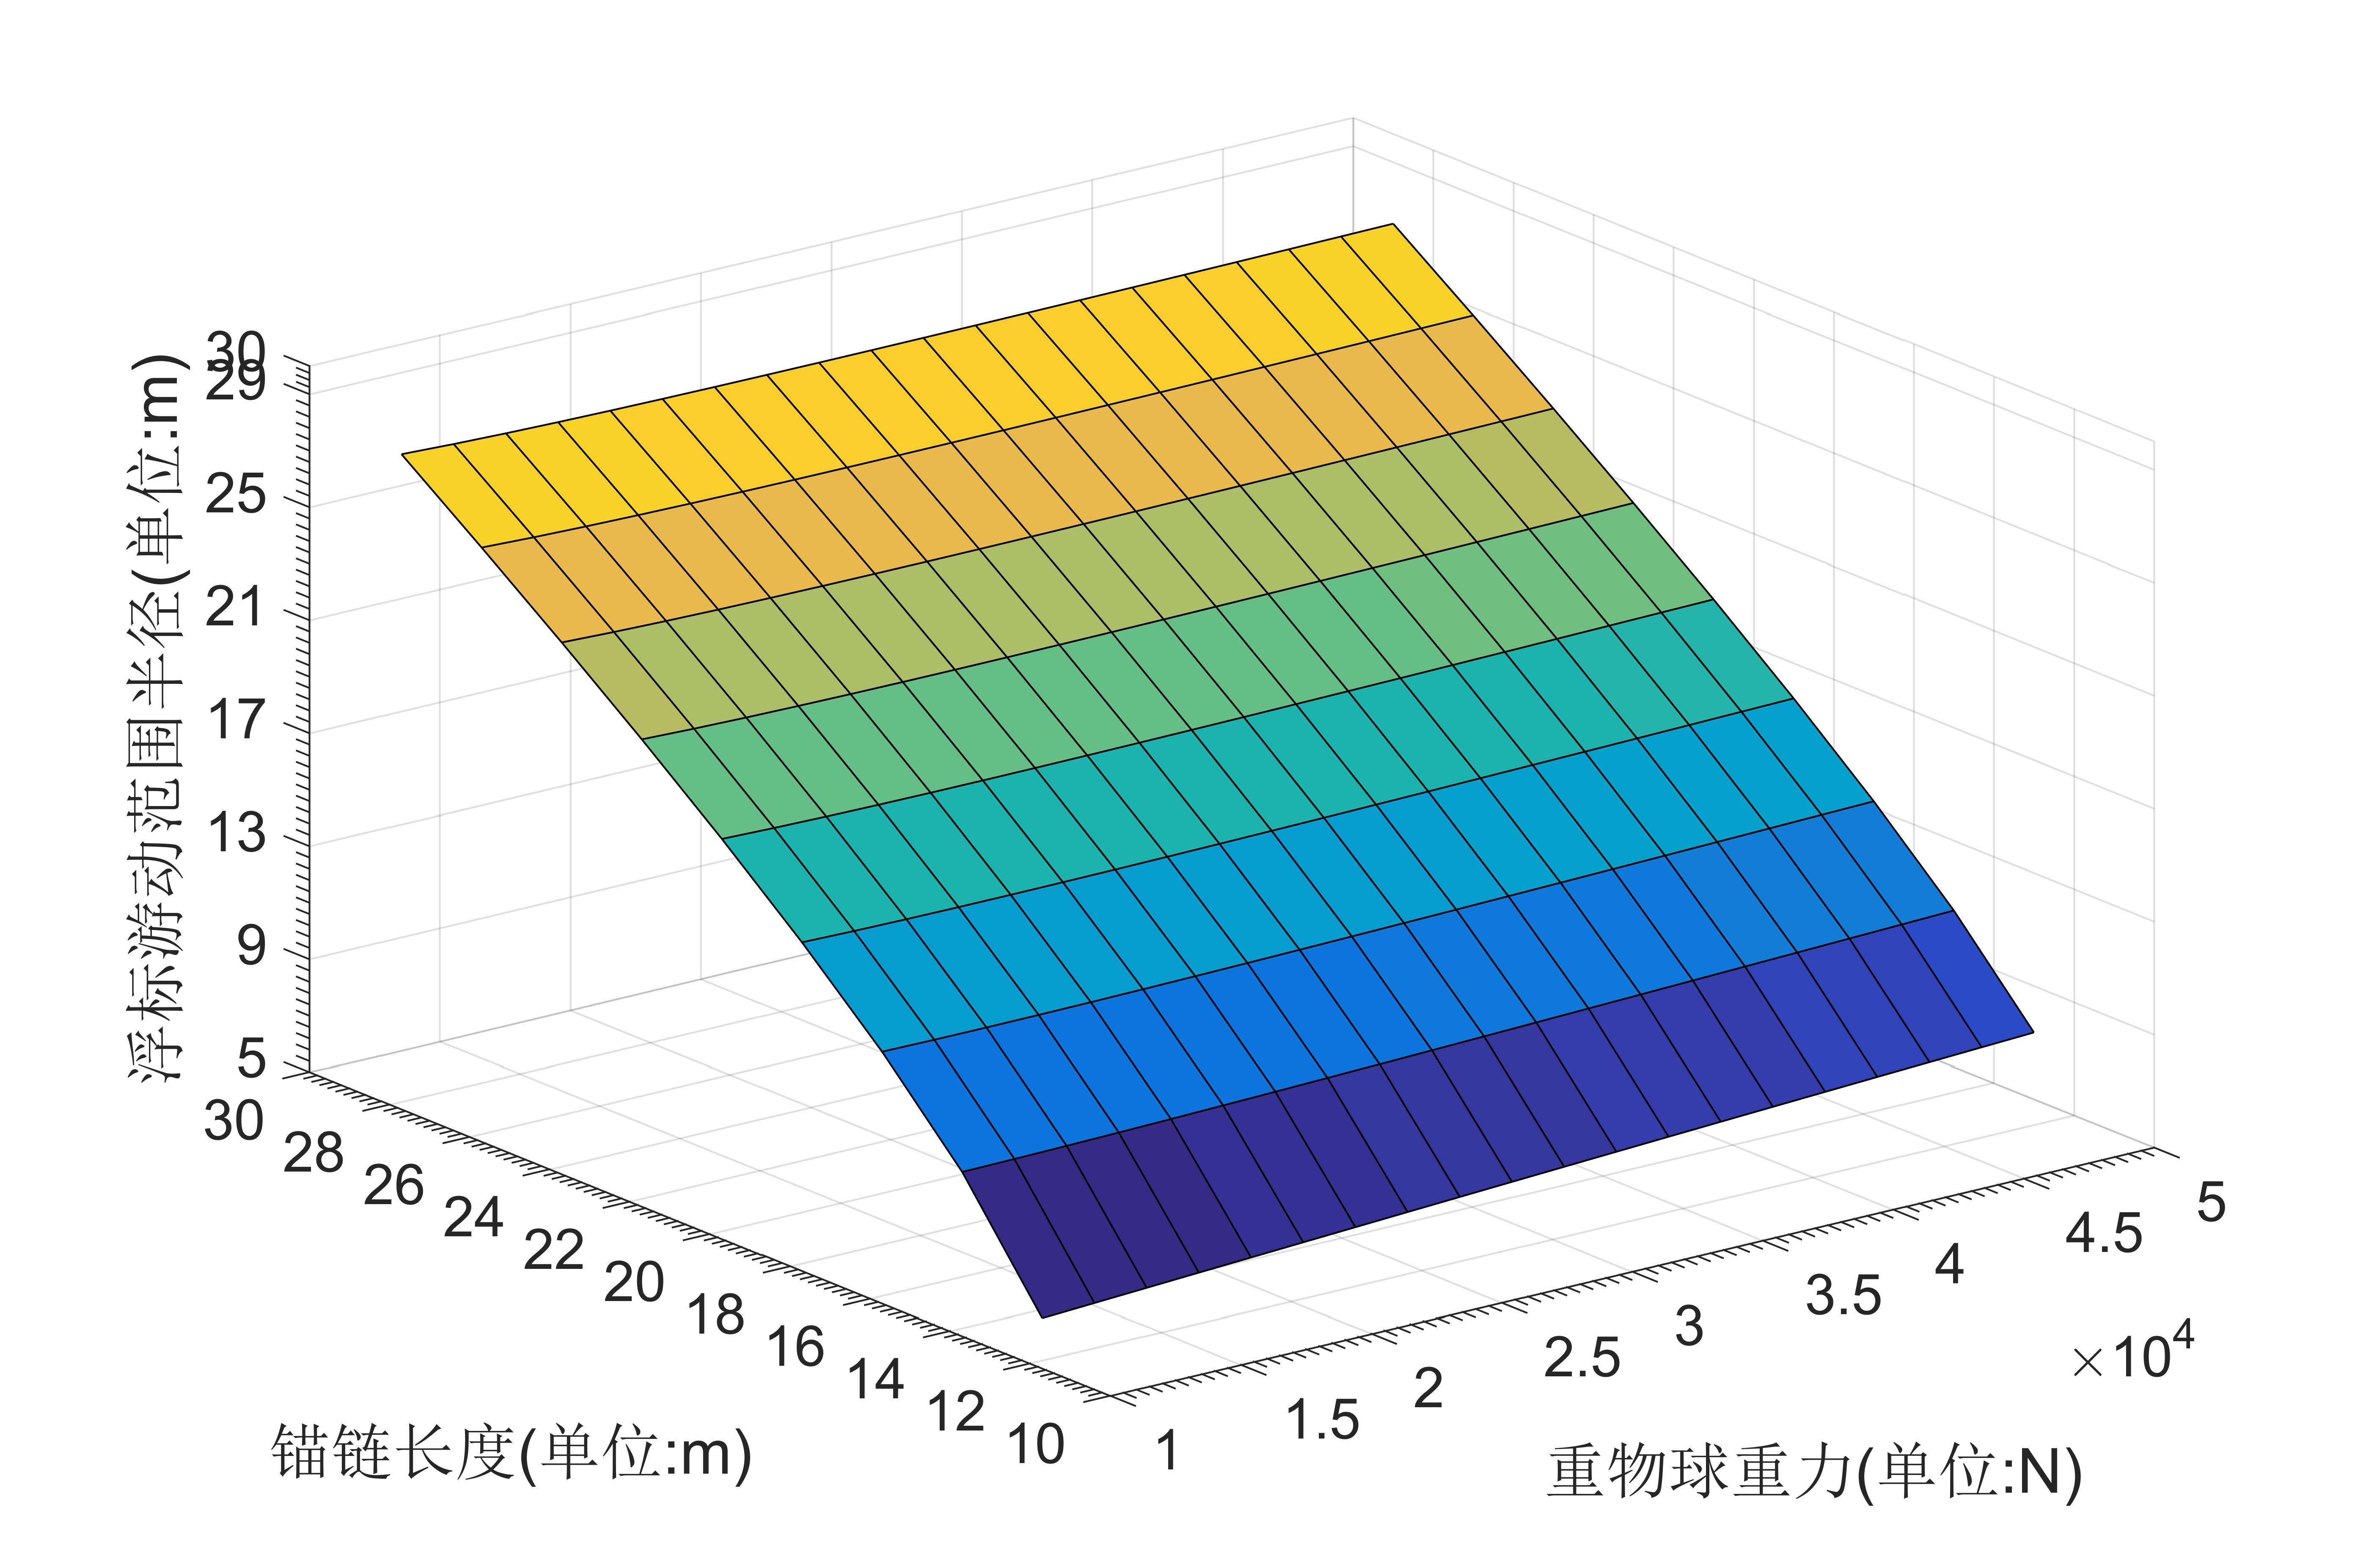
\includegraphics[width=\textwidth]{img/II_18_distance.jpg}   
      \caption{$distance$变化图}   
      \label{fig:2_18_distance}   
    \end{minipage} 
\end{figure}
记重物球重力为$x$轴,锚链长度为$y$轴,各变化量为$z$轴,且正向均为增大的方向。\textbf{可行域}为满足限定条件$\theta\le 5,\beta\le 16$ 的区域。\par 
简单地观察各图易知,每个图总会在$x$方向或$y$方向变化不大,而几乎仅仅受某一变量的影响。这就导致我们可以简单地确定可行解域的大体位置,如图\ref{fig:2_18_theta}中,由$\theta\le 5$条件限制的可行解域即为整个遍历范围的右侧一部分;如图\ref{fig:2_18_theta}中,由$\beta\le 16$条件限制的可行解域即为整个遍历范围的上侧一部分。(此处以x轴正方向为右,y轴正方向为上)两者交叉即得可行解域大致为整个遍历范围的右上角一部分。我们可以通过绘制等高线的方法直观地将这片区域表示出来,如图\ref{fig:II_7_contour1}所示:\par
 \begin{figure}[H]
 	\centering
 	\includegraphics*[width=0.8\textwidth]{img/II_7_contour1}
 	\caption{关于钢桶倾斜角和锚链底端切线水平夹角的双重等高线图}
 	\label{fig:II_7_contour1}
 \end{figure}
从图中可以看到$\theta =5$的等高线变化幅度不是很大,$\beta =16$的等高线有一定倾斜度,因此我们把可能最优解域定为两等高线交点右侧$\beta$等高线上的点。\par 
进一步分析另外两个目标变量,在可行解域上,$h$可近似认为仅随$x$的减小而增大,\\$distance$可近似认为仅随$y$的减小而减小。因而为了使$distance$尽可能小,可能的最优解一定在可行解域的下部边界上。\par 
再考虑边界上的最优解。由于$\theta $与$h$关于$x$的变化方向相反,而两者又都是需要优化的量,故必须确定一个新的目标量将这两者综合起来考虑。题目中没有给出两者的权重分配如何,我们采用赋权值的多目标规划模型\cite{mathmodel},转化为单一目标规划,目标函数定义如式\ref{target_function}:
\begin{equation}
	V_{target} = \frac{1}{2}\cdot (\frac{\theta}{5}+\frac{2-h}{2})
	\label{target_function}
\end{equation}
综上所述,对于某一个特定条件,即水深、锚链型号固定的情况,寻找其锚链长度和重物球重量的最优解的算法如下:\par 
\begin{enumerate}
	\item 遍历两个变量的所有合理值,作出两条等高线
	\item 用两条等高线的数据线性拟合为两个直线方程,用这两个方程求出两条等高线的交点。
	\item 遍历交点右侧$\beta$等高线的目标函数\ref{target_function}值,作出下凸函数图像,求出最小值点的横纵坐标,即为最优解。
\end{enumerate}
现在我们考虑不同锚链型号和不同水深对最优解以及最优解条件下游动区域的影响,使用以上算法求出数据如下:
\begin{table}[!htp]
	\centering
	\caption{重物球重力$(\times10^4N)$}
	\label{table:gravity}
	\centering
	\begin{tabular*}{0.55\textwidth}{c|ccc}
		\hline
		\diagbox[dir=SE]{锚链型号}{水深$m$} & 16 & 18 & 20 \\
		\hline
		\uppercase\expandafter{\romannumeral1} & 4.6410 & 4.6357 & 4.6324\\
		\uppercase\expandafter{\romannumeral2} & 4.6207 & 4.5361 & 4.5305\\
		\uppercase\expandafter{\romannumeral3} & 4.5163 & 4.5065 & 4.4238\\
		\uppercase\expandafter{\romannumeral4} & 4.3991 & 4.3831 & 4.3712\\
		\uppercase\expandafter{\romannumeral5} & 4.3671 & 4.2529 & 4.2283\\
		\hline
	\end{tabular*}
\end{table}
\begin{table}[H]
	\centering
	\caption{锚链长度 $(m)$ }
	\label{table:chain_length}
	\centering
	\begin{tabular*}{0.51\textwidth}{c|ccc}
		\hline
		\diagbox[dir=SE]{锚链型号}{水深$m$} & 16 & 18 & 20 \\
		\hline
		\uppercase\expandafter{\romannumeral1} & 24.67 & 28.90 & 32.91\\
		\uppercase\expandafter{\romannumeral2} & 20.77 & 24.16 & 27.33\\
		\uppercase\expandafter{\romannumeral3} & 17.98 & 20.80 & 23.54\\
		\uppercase\expandafter{\romannumeral4} & 16.05 & 18.59 & 21.01\\
		\uppercase\expandafter{\romannumeral5} & 14.61 & 16.99 & 19.26\\
		\hline
	\end{tabular*}
\end{table}
\begin{table}[H]
	\centering
	\caption{评价函数}
	\label{table:judge_function}
	\centering
	\begin{tabular*}{0.62\textwidth}{c|ccc}
		\hline
		\diagbox[dir=SE]{锚链型号}{水深$m$} & 16 & 18 & 20 \\
		\hline
		\uppercase\expandafter{\romannumeral1} & 0.861395 & 0.861392 & 0.861391\\
		\uppercase\expandafter{\romannumeral2} & 0.861404 & 0.861408 & 0.861395\\
		\uppercase\expandafter{\romannumeral3} & 0.861391 & 0.861402 & 0.861399\\
		\uppercase\expandafter{\romannumeral4} & 0.861405 & 0.861391 & 0.861414\\
		\uppercase\expandafter{\romannumeral5} & 0.861410 & 0.861394 & 0.861401\\
		\hline
	\end{tabular*}
\end{table}
\begin{table}[H]
	\centering
	\caption{游动半径$(m)$}
	\label{table:distance}
	\centering
	\begin{tabular*}{0.5\textwidth}{c|ccc}
		\hline
		\diagbox[dir=SE]{锚链型号}{水深$m$} & 16 & 18 & 20 \\
		\hline
		\uppercase\expandafter{\romannumeral1} & 23.21 & 26.94 & 30.41\\
		\uppercase\expandafter{\romannumeral2} & 18.89 & 21.61 & 24.06\\
		\uppercase\expandafter{\romannumeral3} & 15.62 & 17.62 & 19.48\\
		\uppercase\expandafter{\romannumeral4} & 13.25 & 14.80 & 16.20\\
		\uppercase\expandafter{\romannumeral5} & 11.35 & 12.63 & 13.74\\
		\hline
	\end{tabular*}
\end{table}
分析表\ref{table:gravity}、表\ref{table:chain_length}、表\ref{table:judge_function}和表\ref{table:distance}中的数据得出以下结论:
\begin{enumerate}
	\item 水深增大,重物球重力和锚链长度都在增大,又因为若想满足两个角度限制的条件,必须选择最大的重物球重力和最长的锚链长度。故对于每个锚链型号,都应选择水深20米时的结果。
	\item 相同水深情况下,锚链密度越大,游动半径越小。
	\item 不管水深和锚链型号为多少,评价函数的值几乎没有差别。
	\item 综合以上两点考虑,最终得出的最优解为长度为19.26米的V型锚链和重力为$42283N$的重物球。
\end{enumerate}
外部条件为风速$36m/s$,水速为$1.5m/s$,水深为$20m$的情况下,求出的各项数据结果如表\ref{table:result_3}和表\ref{table:pipe_angle_3}所示:
\begin{table}[!htp]
	\centering
	\caption{问题三部分计算结果}\label{table:result_3}
	\centering
	\begin{tabular*}{0.8\textwidth}{ccccc}
		\hline
		风速$(m/s)$ & 钢桶倾斜角$(^\circ)$ & 吃水深度$(m)$ & 游动半径$(m)$ & 锚链参数$a$ \\
		\hline
		36 & 4.1441 & 1.7911 & 14.3234 & 48.8752\\
		\hline
	\end{tabular*}
\end{table}
\begin{table}[H]
	\centering
	\caption{问题一钢管倾斜角计算结果}
	\label{table:pipe_angle_3}
	\begin{tabular*}{0.82\textwidth}{ccccc}
		\hline
		风速$(m/s)$ & 钢桶倾斜角1 & 钢桶倾斜角2 & 钢桶倾斜角3 & 钢桶倾斜角4\\
		\hline
		36 & 0.99743 & 0.99742 & 0.99741 & 0.99740\\
		\hline
	\end{tabular*}
\end{table}

\section{模型总结}

\subsection{模型优点}

\begin{enumerate}

\item 由于本模型通过求解物理力学方程以及悬链线方程得到解,只需输入外部条件参数和锚链型号即可给出需要的重物球重量和锚链长度。对于问题一类型的问题可以快速求解。

\item 当一个参数不确定时,可以通过二分法求解出其范围,得到最优解。对于问题二类型的问题也可以快速地得到解决。

\item 对于问题三,本模型采用基于加权系数法和优先等级法的多目标规划模型,逐步排除了某些自变量对某些维度的影响,并且将某些目标量合并为一种目标量,极大降低了模型复杂度,提高了求解速度。

\end{enumerate}

\subsection{模型缺点}

\begin{enumerate}
\item 本模型建立在优先等级法之上,这种方法本身可能会导致模型落入局部最优解。
\item 对于加权系数法的权值设定过于简单,没有考虑真正的实际情况,而直接做相同比重处理。这样会可能导致对某一要素的优化程度过低。
\item 模型中使用拟合曲线对数据进行拟合时可能输入数据范围太小,或应该使用高次多项式拟合和非线性拟合,以达到更好地效果。
\end{enumerate}


\bibliographystyle{plain}
\bibliography{ref}

\newpage
\appendix
\textbf{附录}
\section{模型求解代码}

\begin{lstlisting}
	% 下标指定:
	% fl 浮标
	% p 钢管
	% b 钢桶
	% s 重物球
	% c 锚链
	format short;
	syms h;% 浮标露出水面高度
	v = 24;% 第一题风速
	u = 1.5;
	d_fl = 2;% 浮标底面直径
	g = 9.8;% 重力加速度
	rho = 1025;% 海水密度
	H = 2;% 浮标高度
	Fw = 0.625*v^2*d_fl*h;% + 374*u^2*d_fl*(H-h);% 水力+风力
	f_fl = rho*g*(H-h)*d_fl^2*pi/4;% 浮力
	G_fl = 1000*g;% 浮标重力
	T(1,:) = [Fw,f_fl-G_fl];% 第一个结点的受力
	% 钢管
	G_p = 10*g;% 钢管重力
	f_p = (1*0.05^2*pi/4)*rho*g;% 钢管浮力
	% T表示六个结点处的受力,其中T(1)到T(5)有递推关系如下:
	for i = 2:5
	    T(i,:) = [T(i-1,1),T(i-1,2)-G_p+f_p];
	end
	% 钢桶
	G_s = 1200*g;% 重物球重力
	f_b = (0.3^2*pi/4)*1*rho*g;% 钢桶浮力
	G_b = 100*g;% 钢桶重力
	% 第六个结点
	T(6,:) = [T(5,1),T(5,2)+f_b-G_b-G_s];% 锚链上端结点受力
	% 锚链上方高度
	for i=1:4
	    temp = (T(i+1,1)+T(i,1))/(T(i+1,2)+T(i,2));
	    t(i) = sqrt(1/(1+temp^2));% t(1~4)为每根钢管倾斜角度的余弦值
	    k(i) = sqrt(temp^2/(1+temp^2));
	end
	temp = (T(6,1)+T(5,1))/(T(5,2)+T(6,2)+G_s);% 钢桶倾斜角度的正切值
	length = sum(t) + sqrt(1/(1+temp^2));% 锚链上方高度
	length2 = sum(k)+sqrt(temp^2/(1+temp^2));%x方向长度投影

	% 锚链
	w = 7*g;%单位长度锚链重力
	R = T(6,1);% 水平方向受力
	L = 22.05;% 锚链长度
	a = R/w;% 悬链线方程参数
	% 以锚链底端为原点,水平方向为横轴,竖直方向为纵轴建立平面直角坐标系
	% 考虑没有铺底的情况
	syms x;% 第六个结点的横坐标
	% 铺底的方法
	x1 = solve(sinh(x/a)==T(6,2)/T(6,1),x);% 将x以h表示
	y1 = a*cosh(x1/a)-a;% 求出第六个结点的纵坐标
	L_right = a*sinh(x1/a);
	% 解方程
	fun1 = matlabFunction(length+y1(1)+H-h-18);
	[hres1,fval1,exitflag1] = fsolve(fun1,1);
	fun2 = matlabFunction(length+y1(2)+H-h-18);
	[hres2,fval2,exitflag2] = fsolve(fun2,1);
	% 通过检验exitflag值,决定哪一个方程有解
	% 判断哪个是解
	if exitflag1<0
	    hres = hres2;
	    flag = 2;
	else
	    hres = hres1;
	    flag = 1;
	end
	L_right = eval(subs(L_right,h,hres));
	if L > L_right
	    %铺底的情况
	    yres = eval(subs(y1(flag),h,hres));% 第六个节点高度
	    L_right = eval(subs(L_right(flag),h,hres));% 锚链在水平线上方的长度
	    x1 = eval(subs(x1(flag),h,hres));% 锚链水平方向长度
	    length2 = eval(subs(length2,h,hres));% 第六个节点上方水平方向长度
	    distance = L-L_right+length2+x1; %水平偏移
	    theta = eval(subs(atan(temp)*180/pi,h,hres));% 钢桶倾斜角度
	    pipetheta = eval(subs(acos(t)*180/pi,h,hres));% 钢管倾斜角度
	    a = eval(subs(a,h,hres));
	    theta
	    pipetheta
	    x1
	    yres
	    hres
	    distance
	else
	    % 不铺底的情况
	    beta = (T(6,2)-w*L)/T(6,1);% 锚链低端切线斜率
	    x2 = solve(beta*cosh(x/a) + sinh(x/a)*(beta^2 + 1)^(1/2)==T(6,2)/T(6,1),x);% 将x以h表示
	    y2 = a*beta*sinh(x2/a) + a*cosh(x2/a)*(beta^2 + 1)^(1/2)-a*sqrt(beta.^2+1);% 求出第六个结点的纵坐标
	    fun1 = matlabFunction(length+y2(1)+H-h-18);
	    hres1 = fsolve(fun1,1.2);
	    fun2 = matlabFunction(length+y2(2)+H-h-18);
	    hres2 = fsolve(fun2,1.2);
	    if isreal(hres1)
	        hres = hres1;
	        flag = 1;
	    else
	        hres = hres2;
	        flag = 2;
	    end
	    betatemp = eval(subs(beta,h,hres));
	    betares = atan(betatemp)*180/pi;% 锚链底部切线与水平线夹角
	    x2 = eval(subs(x2(flag),h,hres));% 第六个结点横坐标
	    length2 = eval(subs(length2,h,hres));% 第六个节点上方水平方向长度
	    distance = length2+x2; %水平偏移
	    theta = eval(subs(atan(temp)*180/pi,h,hres));% 钢桶倾斜角度
	    yres = eval(subs(y2(flag),h,hres));% 第六个节点纵坐标
	    pipetheta = eval(subs(acos(t)*180/pi,h,hres));% 四个钢管的倾斜角
	    a = eval(subs(a,h,hres));% 悬链线参数
	    theta
	    pipetheta
	    x2
	    yres
	    hres
	    a
	    pipetheta
	    betatemp
	    betares
	end
\end{lstlisting}

\section{二分法搜索代码}
\begin{lstlisting}
% 对指定参数进行二分法搜索
function result = qsearch()
	result=zeros(20,3);
    left = 2500*9.8;right = 3500*9.8;
    % 迭代次数为20
	for i = 1:20
        x = (left+right)/2;
        [a,b]=t2(x);
        result(i,2:3)=[a,b];
        result(i,1)=x/1000;
        if a>0
            left = x;
        else
            right = x;
        end
    end
end
\end{lstlisting}

\section{问题三代码}
\begin{lstlisting}
	clear;clc;
	result = zeros(3,3);
	for depthindex = 1:3
	    m = 20:1:30;mi=size(m);mi=max(mi);
	    n = 30000:1000:40000;ni=size(n);ni=max(ni);
	    H = zeros(mi,ni);
	    D = zeros(mi,ni);
	    T = zeros(mi,ni);
	    B = zeros(mi,ni);
	    for i = 1:mi
	        for j = 1:ni
	            [hres,distance,theta,betares,xres,yres] = t3(m(i),n(j),14+depthindex*2);
	            H(i,j) = hres;
	            D(i,j) = distance;
	            T(i,j) = theta;
	            B(i,j) = betares;
	        end
	    end
	    [x,y] = meshgrid(n,m);
	    figure(depthindex*2-1);
	    v1 = [5,5];
	    [Ct1,ht1] = contour(x,y,T,v1);
	    clabel(Ct1,ht1);
	    x1 = Ct1(1,:);y1 = Ct1(2,:);
	    y1(x1<35000) = [];x1(x1<35000)=[];
	    y1(x1>36000) = [];x1(x1>36000)=[];
	    a = polyfit(x1,y1,1);
	    hold on;
	    v2 = [4,7];
	    [Ct2,ht2] = contour(x,y,T,v2);
	    clabel(Ct2,ht2);
	    v3 = [16,16];
	    [Cb1,hb1] = contour(x,y,B,v3);
	    x2 = Cb1(1,:);y2 = Cb1(2,:);
	    y2(x2<35000) = [];x2(x2<35000)=[];
	    y2(x2>36000) = [];x2(x2>36000)=[];
	    k = polyfit(x2,y2,1);
	    clabel(Cb1,hb1);
	    v4 = [10,22,28];
	    [Cb2,hb2] = contour(x,y,B,v4);
	    clabel(Cb2,hb2);
	    syms t;
	    xres = solve(a(1)*t+a(2)==k(1)*t+k(2),t);
	    xres = max(xres);
	    yres = k(1)*xres+k(2);
	    xres=eval(xres);
	    yres = eval(yres);
	    plot(xres,yres,'.');
	    [hres,distance,theta,betares,x6,y6] = t3(yres,xres,14+depthindex*2);
	    x3 = linspace(xres,50000,20);
	    num = max(size(x3));
	    y3 = k(1)*x3+k(2);
	    evalfunc = zeros(1,num);
	    for j = 1:num
	        [hres,distance,theta,betares,x6,y6] = t3(y3(j),x3(j),14+depthindex*2);
	        evalfunc(j) = (theta/5+(2-hres)/2)/2;
	    end
	    figure(depthindex*2);
	    plot(x3,evalfunc);
	    [val_opt,index] = min(evalfunc);
	    x_opt = x3(index);
	    y_opt = y3(index);
	    result(depthindex,:) = [x_opt,y_opt,val_opt];

	end

	result
\end{lstlisting}

\end{document}